%% Thesis template conforming to Williams College rules.
% Thanks to Ben Wood '08 and other contributors.
%
\documentclass[oneside]{report}

\usepackage[top=1.0in, bottom=1in, left=1in, right=1in, includehead]{geometry}
\pagestyle{headings}
\usepackage{setspace}

%% Special math fonts and symbols
\usepackage{amssymb}
\usepackage{amsfonts}
\usepackage{amsmath}
\usepackage{amsthm}

%% Rotate tables and figures
\usepackage{rotating}

%% Used for TODO items
\usepackage{color}
\usepackage{todonotes}
\newcommand{\todoi}[1]{\todo[inline, color=blue!20]{TODO: {#1}}}

%% used for code listings.
\usepackage{float}

%% Used to replace LaTeX's ugly emptyset with diameter, which looks nicer.
\usepackage{wasysym}

%% Nicely formatted algorithms.
\usepackage{algorithmicx}
\usepackage[chapter]{algorithm}
\usepackage{algpseudocode}

%% Nicely formatted listings.
\usepackage{xcolor}
\usepackage[defaultmono]{droidsansmono}
\usepackage{listings}
\usepackage{etoolbox}

% Display language after listings box
\makeatletter
\AtEndEnvironment{lstlisting}{\xdef\xlang{\lst@language}}
\AfterEndEnvironment{lstlisting}{\begin{flushright}\vspace{-8mm}\texttt{\xlang}\end{flushright}}
\makeatother

\newcommand{\ocamlcommentstyle}{\color{blue}}

% OCaml listing definition: https://gitlab.inria.fr/fpottier/visitors/blob/c54b05ddf255ba50e89943f165b9da7de0ceb3f9/doc/listings-ocaml.tex
\lstdefinelanguage{ocaml}[Objective]{Caml}{
  % Fix errors in the default definition of ocaml.
  deletekeywords={closed,ref},
  morekeywords={initializer},
  % General settings.
  flexiblecolumns=false,
  showstringspaces=false,
  framesep=5pt,
  commentstyle=\ocamlcommentstyle,
  % By default, we use a small font.
  basicstyle=\tt\small,
  numberstyle=\footnotesize,
  % LaTeX escape.
  escapeinside={$}{$},
}
% Shell listing definition: https://tex.stackexchange.com/questions/310335/using-bash-listings-to-bold-variables-and-functions
\lstdefinelanguage{bash}%
  {morekeywords={awk,break,case,cat,cd,continue,do,done,echo,elif,else,%
      env,esac,eval,exec,exit,export,expr,false,fi,for,function,getopts,%
      hash,history,if,in,kill,login,newgrp,nice,nohup,ps,pwd,read,%
      readonly,return,set,sed,shift,test,then,times,trap,true,type,%
      ulimit,umask,unset,until,wait,while,source},%
   morecomment=[l]\#,%
   morestring=[d]",%
   alsoletter={*"'0123456789.},%
   alsoother={\{\=\}},%
   literate={{=}{{{=}}}1},%
   literate={\$\{}{{{{\bfseries{}\$\{}}}}2,%
   otherkeywords={ [, ], \{, \} }%
  }[keywords,comments,strings]%

\lstdefinelanguage{shard}%
  {morekeywords={awk,break,case,cat,cd,continue,do,done,echo,elif,else,%
      env,esac,eval,exec,exit,export,expr,false,fi,for,function,getopts,%
      hash,history,if,in,kill,login,newgrp,nice,nohup,ps,pwd,read,%
      readonly,return,set,sed,shift,test,then,times,trap,true,type,%
      ulimit,umask,unset,until,wait,while,
      cluster,source},%
   morecomment=[l]\#,%
   morestring=[d]",%
   alsoletter={*"'0123456789.},%
   alsoother={\{\=\}},%
   literate={{=}{{{=}}}1},%
   literate={\$\{}{{{{\bfseries{}\$\{}}}}2,%
   otherkeywords={ [, ], \{, \} }%
  }[keywords,comments,strings]%

\lstset{
    language=ocaml,
    basicstyle=\ttfamily\small,
    aboveskip={1.0\baselineskip},
    belowskip={1.0\baselineskip},
    columns=fixed,
    extendedchars=true,
    breaklines=true,
    tabsize=4,
    prebreak=\raisebox{0ex}[0ex][0ex]{\ensuremath{\hookleftarrow}},
    frame=lines,
    showtabs=false,
    showspaces=false,
    showstringspaces=false,
    keywordstyle=\color[rgb]{0.627,0.126,0.941},
    commentstyle=\color[rgb]{0.133,0.545,0.133},
    stringstyle=\color[rgb]{01,0,0},
    numbers=left,
    numberstyle=\small,
    stepnumber=1,
    numbersep=10pt,
    captionpos=t,
    escapeinside={\%*}{*)},
}

%% More kinds of arrow with stuff
\usepackage{empheq}\usepackage{multicol}
\usepackage{subfigure}

%% URLs
\usepackage{hyperref}

%% Advanced tables
\usepackage{tabularx}
\usepackage{multirow}

%%%%%%%%%%%%%%%%%%%%%%%%%%%%%
%% Thesis body %%
%%%%%%%%%%%%%%%%%%%%%%%%%%%%%

\begin{document}

%%%%%%%%%%%%%%%%%%%%%%%%%%%%%
%% Title page              %%
%%%%%%%%%%%%%%%%%%%%%%%%%%%%%

\begin{titlepage}
  $\;$
  \vskip1.5in
  \onehalfspacing
  \begin{center}
    {\LARGE
      Shard : Ad hoc, Reliable, Distributed Shell
    }
    \large
    \vskip.25in
    by\\
    Markus Feng\\
    \vskip.125in Professor Daniel W. Barowy, Advisor\\
    \vskip.125in Professor Jeannie Albrecht, Advisor\\
    \singlespacing\vskip.375in
    \small
    A thesis submitted in partial fulfillment\\
    of the requirements for the\\
    Degree of Bachelor of Arts with Honors\\
    in Computer Science\\
    \vskip.5in
    Williams College\\
    Williamstown, Massachusetts\\
    \vskip.5in
    \today
    %%\vskip.5in
    %%{\Huge \textbf{DRAFT}}
  \end{center}
\end{titlepage}

%%%%%%%%%%%%%%%%%%%%%%%%%%%%%

\tableofcontents
\listoffigures
\listoftables
\onehalfspacing

\chapter*{Abstract}

Performing tasks that are distributed among many systems currently fail to achieve each of the goals of being reliable, easy to set up, closely resembling an existing technology, and friendly to users without distributed systems knowledge.
Because distributed systems are inherently unreliable, succeeding in these goals require the system to provide an abstraction for error handling and recovery that account for the many failure cases that may arise.
This thesis project attempts to define a set of error handling semantics that is simple to use, but powerful enough to be applied to a diverse set of use cases.
We demonstrate the utility of these semantics by implementing a shell-based programming language, Shard.
Using this language, anyone with basic shell knowledge should be able to write and run scripts that runs over multiple machines reliably.
The Shard language will greatly aid in increasing the accessibility and simplifying the process of running distributed programs in domains including systems administration and scientific computing.


\chapter*{Acknowledgments}

I could not have written this thesis without the help of my advisors, Dan Barowy and Jeannie Albrecht, who have both been invaluable in guiding me along in the process. Special thanks to both Dan and Jeannie for taking me on as a thesis student during their sabbatical leaves, at a time when the everyone's world has been affected by the COVID-19 pandemic, helping me with ideas, advice, editing, and making sure that I end up meeting certain deadlines. In addition, I would like to acknowledge all of my family and friends, including the Williams Jesup community, who have supported me in these times.

%%%%%%%% Chapters %%%%%%%%%%%%

%% Introduction
\chapter{Introduction}

\section{Motivation}
% \begin{itemize}
%   \item What makes this project unique (will elaborate in background)
%   \item Introduce three pillars (distributed, reliable, easy to use)
% \end{itemize}

The ability to run a program or task over a network is useful for programmers and computer users in many situations, particularly because of increasing popularity in moving computational resources to the cloud or remote datacenters.
Many developments in distributed computing focus on designing and implementing systems that work well in a large-scale, complex, scalable, and highly performant environment, as discussed in the \textbf{Background} chapter.

Frequently, the trade-off for these systems is that powerful, reliable distributed systems involve  complicated configuration and error handling to sure that they work in the first place, trading away simplicity in return for utility, making it often take a disproportionate amount of effort to perform a simple task in a distributed manner.
Examples of configuration needed in these systems include adding IP address whitelists, opening ports, installing and configuring the distributed platform on each machine, setting up external dependencies, creating a large project for each program, and tuning various parameters, just to name a few.

This thesis describes the design and implementation of the Shard distributed framework, designed to make it easy for any programmer to create and run a distributed program with minimal configuration, regardless of the programmer's background in distributed systems. The Shard distributed framework includes the Shard programming language, which extends the shell programming language by abstracting away the distributed system and automatically handling any errors that may occur in the running of the program as a result of failures in the distributed system.

We have defined three \textit{core pillars} that combine to describe the goals of Shard: it should be distributed, reliable, and easy to use. Our claim is that Shard is specifically designed to achieve the goals set by each of the three core pillars, whereas most computing systems only satisfy at most two out of the three pillars.
In the following section, we describe each of the core pillars in more detail, including why the core pillar is important in achieving the goals of Shard.

\subsection{Distributed}
% \begin{itemize}
%   \item Why would someone want a distributed program?
%   \item What are some challenges of a distributed program?
%   \item Talk about error handling, segue into reliability
% \end{itemize}

The first core pillar of Shard is that it is distributed.
This means that a Shard program should be able to interact with a set of many computers, which by default are assumed to be located across a network boundary.
Shard is explicitly designed to make it easy for parts of a program to be distributed, with syntax-level support for running parts of the code on the distributed system that seamlessly integrate with language features.
A typical Shard program that utilizes the distributed system should not be significantly more complex than a comparable program that performs all of its computations locally.

There are many reasons why a distributed program may be wanted or beneficial.
One example of why a program may want to be distributed is that a program wishes to use resources on other machines across a network, where the remote machine may have more abundance or even exclusive access to certain resources.
These include hardware resources such as CPUs, GPUs, or special purpose hardware; software resources such as the presence of certain operating systems, programs, or libraries; and data resources such as databases and other data stores.

Another example of a program that benefits from being distributed is a program that wishes to perform a certain task on a specific set of machines, such as installing packages, collecting logs, or configuring the system.

Most programming languages are not designed to seamlessly support distributed computing.
Assumptions are made that the program is run entirely on one machine (and sometimes even a single core), and adding distributed features to an existing program may involve rewriting large parts of the original program, including clunky external dependencies, or restricting the program to limited functionality within the programming language.

One reason why distributed computing support is limited among languages is that there are numerous difficulties that arise specifically in distributed systems. Some of these include discovery of remote systems, connecting to the system, data transfer, system state serialization, and concurrency.
% cite from somewhere? unsure
One difficulty in particular is the problem of error handling, as a distributed system is inherently unreliable. This will be addressed in more detail in the description of the next core pillar, reliability.

A notable programming language that includes specific fault-tolerant distributed systems support is Erlang \cite{armstrong2010erlang}. Erlang uses the approach of message passing between processes as the method of inter-process communication, in which processes on a distributed network can participate in a single application using this message passing approach, tackling both the issues of concurrency and parallelism.
However, this approach requires programmers to learn a completely new style of programming when working with distributed programs, and thus is not used in Shard.

% \todoi{Future: Talk about Go; goroutine does not quite do the same thing}

Instead, Shard builds on top of the shell programming language, specifically the POSIX shell, which is described in more detail in the \textbf{Command-line Shells} section of the \textbf{Background} chapter. Many extensions of the POSIX shell are widely used by system administrators, programmers, and other computer users, who are accustomed to using these programs when interacting with the computer.

Notably, the POSIX shell does not contain special support for distributed computing. Shard is designed to be a superset of the POSIX shell, with additions to its syntax, semantics, and built-in functions that result in direct support for distributed computation, allowing Shard to satisfy the core pillar of being distributed.

\subsection{Reliable}
% \begin{itemize}
%   \item Error handling
%   \item Why is reliability important?
%   \item Segue - how does it tie into being easy to use
% \end{itemize}

The second core pillar of Shard is that it should be reliable.
This means that Shard should make a best-effort attempt to complete the distributed computing task that is assigned to it.
Shard should be able to internally handle any errors encountered during the execution of the distributed program, such as a temporary or permanent failure to connect to a host, or loss of data along the way, only exposing the error to the user when the failure cannot be overcome.
This means that using Shard should result in a more reliable experience than the reliability of the underlying distributed system itself.

In general, this core pillar is much more difficult to satisfy for distributed programs compared to non-distributed programs, because while non-distributed computer programs are expected to be reliable in executing an average set of instructions, barring some exceptional circumstance, distributed programs work in the opposite manner, where reliability is assumed not to hold.

The specific reasons why distributed systems are unreliable are explained in more detail in the \textbf{Distributed Computing} section of the \textbf{Background} chapter, but the basic summary is that distributed systems work on top of an ultimately unreliable network, and each machine in the system having a chance of failure means that it is significantly more likely for the entire system to have one or more failures in total.

This pillar needs to be addressed by Shard in particular because many simple computer systems that satisfy the other two pillars of being distributed and easy to use fail to satisfy this pillar, which causes the system to be less useful in practice, where failures in the distributed system often occur.
For example, the examples mentioned in the \textbf{Distributed Command-line Shells} section of the \textbf{Background} chapter generally focus on performing the distributed task on the machines in the distributed cluster, but do not provide special handling to circumstances when one or more of the tasks fail to complete.

Reliability is important because it allows Shard programs to be more predictable and deterministic, characteristics that are desirable for most computer programs. If reliability were not a part of the platform itself, then every program using the platform would have to include extra code to cover for any problems that occur, which can end up being inefficient, time-consuming, and error-prone itself. On the other hand, building error-handling mechanisms at the platform-level as Shard does can provide reliability to all programs on that platform without extra or special care.

\subsection{Easy to use}
% \begin{itemize}
%   \item Ease of use
%   \item Ad-hoc
%   \item Low knowledge barrier
%   \item Why is being easy to use important?
%   \item Distinguishes Shard from other projects
% \end{itemize}

The third core pillar of Shard is that it should be easy to use.
This means that Shard should be useful in an ad hoc situation for any programmer to run a distributed program.
Shard should be easy to use for someone with little to no background knowledge in distributed computing and in Shard itself, so from a language design standpoint, it should be as clear as possible in both reading a Shard program to understand what it does, and in creating a Shard program to complete a certain task.
Shard should be also be easy to use on any single machine that is supported along with any cluster of machines used to perform a distributed computation on, with minimal amounts of installation and configuration on both the machine starting the Shard program and the machines in the cluster
This minimal configuration and installation should be simple and also not require sophisticated background knowledge to perform.
It should be fast and easy to get from the point of Shard being installed to running the program on Shard, particularly for someone who has already used Shard before.

There are clear benefits to a computer system being easy to use.
From the standpoint of having a low knowledge barrier, ease of use can mean that the system is useful to a larger audience of users, since the barrier of learning a new tool or its prerequisite background knowledge may stop larger numbers of people from trying it out in the first place, resulting in the system only being useful for a small niche of trained experts, even if the ultimate benefit of using the system is greater than the learning cost.
In addition, Shard being easy to use may mean that it is a better tool for ad hoc situations, where the goal is to solve a problem of running a distributed program using some combination of the least effort and the least time, which can give it a significant edge over more powerful but heavyweight distributed systems, where time is wasted setting up the system or writing the distributed program.

The core pillar of being easy to use is what separates Shard from many traditional distributed systems that will be described in the \textbf{Distributed Computing} section of the \textbf{Background} chapter, and which do follow the other two core pillars of being distributed and reliable. For many of those systems, it is plausible that the time it takes to get the system up and running is many times longer than the time it takes to install Shard, write the Shard program, run the Shard program, and complete the task.

\section{Summary}
% \begin{itemize}
%   \item What my project is
%   \item What I've done
%   \item How I've done it
%   \item Measurement of success
% \end{itemize}
% \begin{itemize}
%   \item Explain the layout of the rest of my thesis
% \end{itemize}

The Shard project's goal is to design and implement a distributed shell programming language that accomplishes the goals outlined by the three core pillars of being distributed, reliable, and easy to use.
The work and evaluation of Shard  will be described in the remainder of the thesis, separated into the following parts:

\begin{sloppypar}
  \textbf{Chapter 2} describes the background of related computer systems, including other non-distributed and distributed command-line shells, and other distributed systems.
\end{sloppypar}

\textbf{Chapter 3} describes the design of the Shard, introducing the concept of application classes and providing details about the design of both the Shard programming language and the network layer used in the communication of the distributed framework.

\textbf{Chapter 4} describes the implementation of Shard, separated into the shell, language, network layer, and application class implementations.

\textbf{Chapter 5} describes the evaluation of the Shard distributed system and how well it achieves the goals of the three core pillars as described in this chapter.

\textbf{Chapter 6} provides a conclusion to this thesis, summarizing the contributions and providing potential directions for future work.


%% Background
\chapter{Background}

In this chapter, we describe the background behind command-line shells, focusing in particular on their relationship with the UNIX operating system and the specification of the POSIX shell.
After that, we provide an overview of distributed computing, with a deeper look at fault tolerance properties that will guide the error handling semantics in Shard, and several examples of distributed systems, including Hadoop, Ganglia, and Plush.
Next, we discuss existing examples of distributed command-line shells, including their features, implementations, and weaknesses.
Finally, we provide a summary of existing shells, distributed systems, and distributed shells, along with how Shard builds upon these existing systems.

\section{Command-line Shells}
\subsection{UNIX Shell}
UNIX is an operating system designed at Bell Labs, with the first versions appearing around 1969-1970 \cite{10.1145/361011.361061}.
UNIX was an influence in many operating systems in use today, with its original form evolving into various BSD distributions (NetBSD, FreeBSD, OpenBSD). The GNU operating system, which is the basis of Linux distributions today, was also designed to be UNIX compatible \cite{bretthauer2001open}.

One of the standard ways of interacting with the UNIX operating system is through a command-line shell \cite{10.1145/361011.361061}.
The operation of the shell involves reading in lines of text typed by the user, interpreting the input as a program of the shell programming language, and performing a command based on the input text.
The most basic command consists of a space-separated list of strings, with the first string being the name of the command, and the remaining strings being the arguments for the command.
The shell searches the file system for the appropriate program to run, based on the name of the command, and feeds the arguments as input to the program.
By default, the standard output of the program is displayed back to the user by the visual interface of the shell program, but indirections can modify this by transferring the output to a file or another program.
When execution completes, control is given back to the user, who can run another command-line command on the shell.
Because the command-line is a program itself, the shell can run itself as a program with the input being a file containing shell commands.
The command-line shell is useful in a wide variety of contexts, in being one of the easiest ways to programmatically interface with the operating system itself, and many operations on computers are able to be performed or even require using shell \cite{10.1145/3371111}.

\subsection{POSIX Shell}
POSIX is a family of IEEE standards originating in the early 1980s that specify a portable operating system interface based on UNIX \cite{10.1145/210308.210315}.
Contained within the POSIX specification is a specification of the POSIX shell, which describes the interface to which the shell command language should conform \cite{posix2017}.
Because each operating system that conforms to the POSIX interface must implement a POSIX shell, there have been a wide variety implementations of POSIX shells on numerous platforms, many of which have additional features that extend the capabilities of the shell.
Popular examples of POSIX-compatible shells include Bash, Dash, Zsh.
The POSIX shell is popular across computing platforms, including even platforms that are not designed to be POSIX compatible, though notably a majority of POSIX shells do not fully conform to the POSIX specification \cite{10.1145/3371111}.
Shard expands on the existing collection of POSIX-compatible shells by adding distributed computing features on top of the existing shell language.

\section{Distributed Computing}

A distributed computing system, or a distributed system, is a computer system that consists of multiple processors on one or more machines that work together but do not directly share memory \cite{10.1145/72551.72552}.
This thesis in particular focuses on multicomputer distributed systems that communicate over a network that is not guaranteed to be reliable.
As such, there may be errors or faults that occur during the operation of the system.

\subsection{Fault Tolerance in Distributed Systems}
There has been significant work in the field of fault tolerant distributed systems, as one important goal in computer systems is to be dependable, which comes with significant challenges when in a distributed environment compared to a program running on a single machine \cite{10.1145/311531.311532}.

% Safety/Liveliness
The two classes of fault tolerance properties in distributed programs are properties of \textit{safety} and \textit{liveliness} \cite{1702415}.
Safety properties ensure that the state of the distributed system never reaches an illegal state, while liveliness properties ensure that the state of the distributed system must eventually reach a completed state.
For example, a safety property of a distributed system may be that one part of a distributed program is not executed until a different part is complete, while a liveliness property of a distributed system may be that the program eventually provides a result, even if one or more machines are stuck in a loop during execution.

% Masking/Fail-safe/Nonmasking
When designating a system to be fault tolerant, it is important to specify which types of faults that the system is tolerant against, and what types of fault tolerant properties are satisfied by the system \cite{10.1145/311531.311532}.
In the strongest form, a system with masking fault tolerance is able to satisfy both safety and liveliness properties against a given set of faults.
Slightly weaker is fail-safe fault tolerance, which ensures safety but does not make liveliness guarantees, capturing the notion that certain illegal states will never appear.
Safety is important in many situations, such as making sure that a missile does not launch in case of individual component failures.
On the other hand, nonmasking fault tolerance, which ensures liveliness but does not make safety guarantees, captures the notion of a system always making progress towards completion, despite the possibility of some amount of incorrect behavior during execution.
Traditionally less focus has been placed on systems in ensuring liveliness compared to ensuring safety, as liveliness issues can be resolved in many cases by manually stopping the system, whereas safety issues can lead to large amounts of damage.

% Potential sections:
% Crash/Fail-stop/Byzantine
% Redundancy
% Error detection and correction

\subsection{Examples}
Fault tolerant distributed systems exist in many forms, with widespread practical usage.
Typically, these systems target solving a specific type of distributed problem, with differences based on the priorities and goals of the individual system.

\subsubsection{MapReduce/Hadoop}
MapReduce is a distributed computation framework developed by Google to handle and process large amounts of data \cite{dean2004mapreduce}.
The data processing is done by splitting up the input into key-value pairs, applying a function in a distributed fashion on each of those value pairs, then using a reduce function to combine the pairs that share a key.
In the implementation used by Google in 2004, a typical MapReduce cluster contained hundreds or thousands of machines.
The problem of making data available to other machines is solved through the use of a distributed file system formed by the disks located at each of the machines in the cluster, which partitions the data storage to individual machines.
Because the data is stored on a particular machine, that same machine can be in charge of performing the necessary map and reduce computations, which optimizes performance.

\begin{sloppypar}
  Apache Hadoop is an open source distributed programming framework that can be used to run MapReduce-style computation on large datasets \cite{Hadoop}.
  Hadoop is designed to target the use case of data processing with extremely large data sets that cannot be handled with ordinary programming techniques that depend on all of the data being available on one machine and the work being done by a single process.
  Hadoop uses a distributed filesystem in a similar manner to Google's MapReduce implementation, with explicit goals of being able to handle faults such as hardware failure, using techniques including replication to make sure that the data is stored reliably across the cluster \cite{borthakur2007hadoop}.
  The fault tolerant properties of Hadoop makes it useful in production usage, where errors are to be expected to occur when dealing with large clusters of machines.
  Both of these systems deal with a problem known as the straggler problem, where a small proportion of the tasks take a much longer time to complete than the remaining tasks.
  The straggler problem is mitigated by reexecuting tasks that are slow to complete, with the hope that the newly executed task will finish faster.
  This must be done while ensuring that the result of the program remains correct.
\end{sloppypar}

Shard borrows some of the ideas from the MapReduce framework in using parts of its programming model for some language features, though its implementation does not intend to mirror all of the exact details of MapReduce.

\subsubsection{Ganglia/GEXEC}
Ganglia is a monitoring system for scalable high-performance distributed programs \cite{MASSIE2004817}.
Ganglia provides an interface for checking and visualizing the status of distributed computation machines, which is useful for organizations and individuals with large scale distributed systems deployments.
One of the central goals of Ganglia is robustness.
Ganglia is designed to monitor failures and continue to operate in the presence of these failures, as individual failures are common in large-scale systems with high resource demands and utilization.
Types of failures as identified by Ganglia include computational, I/O, and network failures on individual machines, along with bottlenecks on a larger scale.

As a monitoring system, it is possible to use the information provided by Ganglia in an application or an application framework.
The utility GEXEC allows executing jobs of machines on a cluster, while providing data and signal forwarding on jobs between the machines \cite{gexec}.
GEXEC supports a mode of operation that utilizes Ganglia, which takes advantage of Ganglia's failure monitoring and handling features to ensure that the system is robust even on large distributed clusters.
Shard is similar to GEXEC in that it can be used to execute jobs on remote machines, but Shard does so in an ad hoc manner, as opposed to requiring the setup of a monitoring service.

\subsubsection{Plush}
Plush is a unified framework for managing various classes of programs to be executed in a wide variety of distributed environments \cite{10.5555/1349426.1349441}.
Like the other distributed system frameworks mentioned above, Plush has an emphasis on detection and recovery from failures through monitoring the state of the system.
Plush acts as a platform for building distributed applications, providing a set of abstractions and configurations to allow error recovery in a user-specified manner, designed in a fashion to be applicable to a wide range of different types of distributed programs.
Shard is similar to Plush in that it is also a platform that abstracts away parts of building distributed programs, though Shard places more of an emphasis on being easily usable by non-experts of distributed systems, while Plush has a more extensive and flexible set of configurations for its remote applications.

\section{Distributed Command-line Shells}
The concept of command-line shells and distributed computing can be combined to form a distributed command-line shell.
A distributed shell is a shell that supports command-line shell features over a distributed cluster of machines.

\subsection{Examples}
The concept of distributed shells has been visited in the past in various forms.
However, none of these shells fully realize the goals of the Shard shell.
In particular, unlike for many of the distributed systems mentioned above, the issue of distributed error handling and recovery is not well addressed by any of the solutions below.

\subsubsection{SSH}
One method of making an ad hoc distributed shell is to invoke the SSH secure shell utility multiple times.
The SSH utility allows users to connect to remote machines over TCP and access the command-line shell on those machines \cite{rfc4251}.
Given a command to run and a list of remote hosts, the shell can iterate over the list, invoke SSH with that remote host as an argument, run the command on the remote host, and finally collect the results back on the local machine.
Notably, this method does not handle error recovery well, or guarantee reliable execution in the event of failures.

\subsubsection{DSH (Dancer's Shell)}
The DSH (Dancer's Shell) Unix program allows the user to send a shell command to all machines in a cluster defined by the user \cite{dshdancer}.
DSH uses an underlying remote execution protocol, such as SSH, for executing shell programs on remote hosts.
The command invocation occurs in a hierarchical fashion, with each node sending the command to some amount of child nodes until the program is executed on all nodes in the cluster.
Notably, for the DSH program, there does not exist an emphasis of reliable execution and error recovery from failures that may arise from the distributed nature of the program.
Other similar implementations of the DSH program exist in various forms, some of them implemented with a different language or work on different platforms.

\subsubsection{Distsh}
Distsh (Distributed Command-Line Interface) is an implementation of a generic distributed shell environment, with steps taken to make accessing a remote machine just like accessing a local one \cite{distsh}.
The Distsh shell language only specifies semantics for connecting to a single remote machine at a time, rather than having the unit of remote computation being a cluster of remote machiens as is the case in DSH.
Similar to DSH, there does not exist error handling semantics to allow reliable execution and error recovery.
The paper specifies that the implementation currently only works when the machine to access is localhost, and there does not appear to have been visible progress on the project since the paper was made public.

\section{Summary}
Command-line shells are an important and useful interface for interacting with a computer.
Therefore, it makes sense to be able to use the command-line shell to interact with many computers simultaneously in a distributed manner.
However, distributed systems come with existing challenges, particularly because failures are much more likely when there are more avenues of failure and more machines that can fail.
While many existing distributed systems have built-in error handling and recovery mechanisms, prior solutions for extending the shell to a cluster of distributed systems do not sufficiently take into account these same errors.
This thesis aims improve upon existing solutions by unifying the reliability built into distributed systems with the simplicity and ease of use of the command-line shell interface.

\chapter{Design}

In this chapter, we discuss the design of the Shard distributed system, which includes the Shard programming language, the Shard network layer, and the Shard application classes that are currently supported.

\section{Overview}
% \begin{itemize}
%   \item High level design
%         \begin{itemize}
%           \item Satisfying the three pillars (ease of use, distributed, reliable)
%           \item Use language to solve problem
%         \end{itemize}
%   \item Separation of design and implementation
% \end{itemize}

Fundamentally, the design philosophy of Shard is to create a computer system that best satisfies the three core pillars, as outlined in the \textbf{Introduction} chapter: being distributed, easy to use, and reliable.

The central design choice of the Shard distributed system is creating a new programming language, rather than writing a library or a set of macros for an existing programming language.
This is primarily due to the ability to provide better syntax level support for the remote execution capabilities of Shard, as the intent is to make writing a distributed program just as easy as writing a local program, in order to better satisfy the ease of use property.
The Shard programming language is built on top of the POSIX shell language, with Shard's syntax and semantics being a direct extension of the POSIX shell.
The POSIX shell is chosen because is widely adopted by programmers on UNIX machines, and the level of familiarity with the language further reinforces Shard's ease of use \cite{posix2017}.
Because of this, in a complete implementation of Shard, almost all valid POSIX shell programs would also be valid Shard programs.

The defining feature of the Shard programming language that separates it from the POSIX shell is the it provides the ability for programs to execute commands on a cluster of remote machines.
The remote commands work similarly to how a subshell works, and are valid Shard programs themselves with the full functionality of the Shard code running locally.

Remote command execution is performed using the Shard network layer, which is designed specifically to work with the Shard shell, and focusing on the core pillars of being distributed and being reliable.
The Shard network layer works by using a pair of communication channels between the local machine where the Shard program originated, and the remote machine where the Shard command should be executed, with messages being passed along the channel to perform the executing of the Shard command on the remote machine, and to ensure this execution is performed in a reliable manner.
A custom network layer is used because it affords Shard full control over ensuring reliability, with a combination of features such as heartbeats, sequence numbers, and retry mechanisms to maximize the reliability of the distributed features of the system.

The Shard network layer also makes it possible to configure its distributed execution so that the functionality is tuned for a certain type of distributed application.
These are known as \textit{application classes} in the Shard distributed system.
The \texttt{single\_command} application class, which executes its program in a best-effort fashion on all machines in the cluster, and the \texttt{data\_parallel} application class, which executes its program many times in parallel on the machines in the cluster and builds on top of a MapReduce-like \cite{dean2004mapreduce} interface.

The various components described in this chapter combine to form the design of the Shard distributed system, without prescribing the way in which this system must be implemented.
Nonetheless, the design of the system is influenced by the practicality of its implementation, which is used to demonstrate the usefulness of the design.
For implementation details, see the \texttt{Implementation} chapter that follows.

\section{Language design}

% \begin{itemize}
%   \item Solves the problem of: ease of use/familiarity
%   \item Describe the programming language
%   \item Based on the POSIX shell standard
%   \item Simple new syntax/semantics for distributed work
%         \begin{itemize}
%           \item Cluster management (builtin)
%           \item Application classes/error handling semantics support
%           \item Run on remote host (@@)
%         \end{itemize}
% \end{itemize}

The Shard programming language is an extension of the POSIX shell programming language, as specified in the POSIX standard \cite{posix2017}.
This means that, by design, Shard contains all of the features in the POSIX shell programming language, and as such, this section will only describe features that are exclusive to Shard.
The Shard programming language is designed primarily to add support for distributed computation to the existing shell programming language, while satisfying the core pillar of being easy to use.

In total, the Shard programming language only adds two features: cluster management and remote execution.
These two language features are enough for Shard to support execution of arbitrarily complicated remote shell programs.
A minimal set of language additions is deliberately chosen to make Shard as similar to the existing POSIX shell as possible, making it easier to learn the language, read existing programs, and write new programs, especially for someone familiar with the POSIX shell.

The syntax of the new features of the Shard programming language are shown in Table \ref{fig:pl_syntax}, with the parameters for the syntax shown in Table \ref{fig:pl_syntax_parameters}.
The semantics of the new features will be explained in detail in the \textbf{Cluster management} and \textbf{Remote execution} sections that follow and supported by examples.

\begin{table}[h]
  \begin{center}
    \begin{tabularx}{\textwidth}{|l|X|}
      \hline
      Feature            & Syntax                                                   \\ \hline
      Cluster management & \texttt{<cluster> ::= cluster -<option> <args>} \newline
      \texttt{| cluster} \newline
      \texttt{<option> ::= a | c | o | p | s | t} \newline
      \texttt{<args> ::= <string>} \newline
      \texttt{| <string> <args>}
      \\ \hline
      Remote execution   &
      \texttt{<remote> ::= (<program>)@@<target>}
      \newline \texttt{| <program>@@<target>}
      \newline \texttt{| (<program>)@@<setting>/<target>}
      \newline \texttt{| <program>@@<setting>/<target>} \newline
      \texttt{<program> ::= <string>} \newline
      \texttt{<setting> ::= <string>} \newline
      \texttt{<target> ::= <string>}
      \\ \hline
    \end{tabularx}
    \caption{Syntax of the Shard programming language features.}
    \label{fig:pl_syntax}
  \end{center}
\end{table}

\begin{table}[h]
  \begin{center}
    \begin{tabularx}{\textwidth}{|l|X|}
      \hline
      Feature            & Parameters                                                                                                                                                                                                                                                                                                                                                                                                                                                                                                                       \\ \hline
      Cluster management & The \texttt{<option>} parameter specifies which cluster built-in command to use. \newline The \texttt{<args>} parameter species the arguments to be passed to the specified cluster built-in command. \newline See Figure \ref{fig:pl_cluster_options} for more details.                                                                                                                                                                                                                                                         \\ \hline
      Remote execution   & The \texttt{<program>} parameter is a legal Shard program, behaving similar to what is allowed in the subshell environment in the POSIX shell. \newline The \texttt{<target>} parameter is either the name of a cluster defined by the cluster management, or a host as accepted by the underlying communication protocol. \newline The \texttt{<setting>} optional parameter may be used by the application class for the cluster; depending on the application class of the cluster, it may be required, optional, or ignored. \\ \hline
    \end{tabularx}
    \caption{Parameters for the syntax of the Shard programming language.}
    \label{fig:pl_syntax_parameters}
  \end{center}
\end{table}

\subsubsection{Example program: Hello, world!}

Before delving into the details about the language, it is informative to look at an example Shard program that uses its remote execution capabilities to print the text ``Hello, world!''.
% This section will conclude with an example Shard program that uses its remote execution capabilities to print the text ``Hello, world!''.

\begin{minipage}[c]{\textwidth-15pt}
  \begin{lstlisting}[language=Shard]
(echo "Hello, world!")@@machine1.cs.williams.edu
\end{lstlisting}
  \smallskip
\end{minipage}

This is one of the simplest examples of a program utilizing remote execution in Shard.
This program uses the \texttt{@@} remote execution operator to run a Shard subprogram on a remote machine, which will be described in detail in the \textbf{Remote execution} section of this chapter.
The program for this remote execution is the program \texttt{echo "Hello, world!"}, which prints the text ``Hello, world!'' to the standard output.
The target for this remote execution is the host \texttt{machine1.cs.williams.edu}.
When this program is run, Shard sends the program \texttt{echo "Hello, world!"} to the remote machine, where it is executed.
The output from the remote machine is redirected to the output of the local machine, where the text ``Hello, world!'' appears on the local standard output, where the Shard command is executed from.

More example programs of specific application classes will come in the \textbf{Application class design} section later this chapter, where the semantics of the application classes in Shard are introduced.

\subsection{Cluster management}
The first feature that Shard adds to its programming language is cluster management.
In Shard, we define a \textit{cluster} as an unordered collection of remote hosts, along with a name and a cluster type.
The cluster type is one of the application classes available to Shard.
Clusters can also have miscellaneous settings configuring the application class.

The Shard programming language adds support for creating and updating clusters, using its \texttt{cluster} builtin function.
A summary of the options for the \texttt{cluster} builtin are shown in Table \ref{fig:pl_cluster_options}.

\begin{table}[h]
  \begin{center}
    \begin{tabularx}{\textwidth}{|l|X|X|}
      \hline
      Option                        & Syntax                                                                                                                                                                                       & Semantics                                                                                                         \\ \hline
      Set                           & \texttt{cluster -s <name>} \newline
      \texttt{<name> ::= <string>}  & Sets the active cluster to the cluster with \texttt{<name>}, creating it if it does not already exist.
      \\ \hline
      Add                           & \texttt{cluster -a <host>} \newline
      \texttt{<host> ::= <string>}  & Adds the host \texttt{<host>} to the active cluster.
      \\ \hline
      Type                          & \texttt{cluster -t <type>} \newline
      \texttt{<type> ::= single\_command} \newline
      \texttt{| data\_parallel}     & Sets the application class of the active cluster to \texttt{<type>}. Valid types specified in the current version are \texttt{single\_command} and \texttt{data\_parallel}.
      \\ \hline
      Option                        & \texttt{cluster -o <key> <value>} \newline
      \texttt{<key> ::= <string>} \newline
      \texttt{<value> ::= <string>} & Sets a configurable option for the active cluster, with the specified \texttt{<key>} to the specified \texttt{<value>}. Valid options depend on the application class of the active cluster.
      \\ \hline
      Clear                         & \texttt{cluster -c}                                                                                                                                                                          & Resets the active cluster, removing all hosts, clearing all options, and setting the cluster type to the default.
      \\ \hline
      Print                         & \texttt{cluster -p <name> | cluster -p} \newline
      \texttt{<name> ::= <string>}  & Prints out the details of the cluster with \texttt{<name>}. If \texttt{<name>} is not specified, instead prints out the details of all clusters.
      \\ \hline
      No arg                        & \texttt{cluster}                                                                                                                                                                             & Prints out the details of all clusters.
      \\ \hline
    \end{tabularx}
    \caption{Options for the \texttt{cluster} builtin function of the Shard programming language.}
    \label{fig:pl_cluster_options}
  \end{center}
\end{table}

The set of clusters defined at any point in time is stored in the shell's environment.
Therefore, shell features that copy the environment, such as subshells, also copy the cluster definitions.
At any given point in time, there is always an active cluster.
By default, if no cluster has been set to be the active cluster, the cluster named \texttt{default} with the default cluster type \texttt{single\_command} is set to the active cluster.
The user can run \texttt{cluster} with the \texttt{-s} (set) option to set the currently active cluster to a cluster with the specified name.
If no cluster with the specified name exists, a new cluster is created.

\begin{minipage}[c]{\textwidth-15pt}
  \begin{lstlisting}[language=Shard]
# Syntax:
# <cluster_set> ::= cluster -s <name>
# Example:
cluster -s testcluster
\end{lstlisting}
  \smallskip
\end{minipage}

Hosts can be added to the active cluster with the \texttt{-a} (add) option.
The specifics behind host resolution is an implementation detail, but IPV4 addresses and ASCII domain names should always be accepted as hosts.

\begin{minipage}[c]{\textwidth-15pt}
  \begin{lstlisting}[language=Shard]
# Syntax:
# <cluster_add> ::= cluster -a <host>
# Example:
cluster -a machine1.cs.williams.edu
\end{lstlisting}
  \smallskip
\end{minipage}

The type of the active cluster can be changed with the \texttt{-t} (type) option.
Valid choices for the cluster type are all of the application classes supported by the implementation of Shard.
As specified in this design, the choices for application classes are \texttt{single\_command} and \texttt{data\_parallel}, with \texttt{single\_command} being the default if none is set.

\begin{minipage}[c]{\textwidth-15pt}
  \begin{lstlisting}[language=Shard]
# Syntax:
# <cluster_type> ::= cluster -t <type>
# <type>         ::= single_command
#                 |  data_parallel
# Example:
cluster -t data_parallel
\end{lstlisting}
  \smallskip
\end{minipage}

Application classes can support specifying options with key-value pairs to modify their behavior. Such options are set for the active cluster with the \texttt{-o} option.

\begin{minipage}[c]{\textwidth-15pt}
  \begin{lstlisting}[language=Shard]
# Syntax:
# <cluster_option> ::= cluster -o <key> <value>
# Example:
cluster -o heartbeat_period 500
\end{lstlisting}
  \smallskip
\end{minipage}

It is possible to clear the active cluster, including its hosts, options, and cluster type using the \texttt{-c} (clear) option.
This results clearing the cluster of all state, returning it to how it was when it was just created.

\begin{minipage}[c]{\textwidth-15pt}
  \begin{lstlisting}[language=Shard]
cluster -c
\end{lstlisting}
  \smallskip
\end{minipage}

Finally, the \texttt{-p} (print) option can be used to print out the details of the cluster to standard output.
Specifically, the output printed by this option should be a list of \texttt{cluster} builtin commands that can be used to reconstruct the state of the specified cluster.
If no cluster name argument is provided, the details of all defined clusters are printed, and if the \texttt{cluster} builtin is called with no arguments at all, it behaves as if it were called with the \texttt{-p} option.

\begin{minipage}[c]{\textwidth-15pt}
  \begin{lstlisting}[language=Shard]
# Syntax:
# <cluster_print> ::= cluster -p <name>
#                  |  cluster -p
#                  |  cluster
# Example:
cluster -a 127.0.0.1
cluster -s cluster1
cluster -a machine1.cs.williams.edu
cluster -a machine2.cs.williams.edu
cluster -t data_parallel
cluster -p cluster1
# Expected output:
# cluster -s "default"
# cluster -a "127.0.0.1"
# cluster -s "cluster1"
# cluster -a "machine1.cs.williams.edu"
# cluster -a "machine2.cs.williams.edu"
# cluster -t "data_parallel"
\end{lstlisting}
  \smallskip
\end{minipage}

Although the \texttt{cluster} builtin does not perform any remote execution by itself, it is essential in specifying the remote hosts, application type, and other options used in the remote execution.

\subsection{Remote execution}
The remote execution language feature is used to execute Shard subprograms on remote machines in a distributed manner.
The language feature consists of a single of syntax addition, revolving around the remote execution operator \texttt{@@}.

\begin{minipage}[c]{\textwidth-15pt}
  \begin{lstlisting}[language=Shard]
# Syntax:
# <remote> ::= <program>@@<target>
#           |  (<program>)@@<target>
# Examples:
ps@@machine1.cs.williams.edu
(echo -n "$(hostname): "; cat /etc/issue)@@testcluster
\end{lstlisting}
  \smallskip
\end{minipage}

The remote program provided can be any valid Shard program, without constraints, making Shard generally useful for running shell code remotely.
The remote target for the program can either be the name of a cluster that has already been defined by Shard, or a host, with the same host resolution policy as that of adding hosts to a cluster.
This Shard subprogram is run on the remote machines in a manner as determined by the application class of the cluster.
If a host is specified, the program will behave as if it were running on a cluster with default settings and the specified host as its only host.

Some application classes, such as \texttt{data\_parallel}, expect a \textit{setting} string in addition to its target.
Similar to the key-value pairs for the cluster \texttt{-o} option, the purpose and behavior of the setting string depends on the specific application class for the cluster, with some application classes completely ignoring the setting string.
Providing an empty string as the setting string is equivalent to not providing a setting string at all.

\begin{minipage}[c]{\textwidth-15pt}
  \begin{lstlisting}[language=Shard]
# Syntax:
# <remote_setting> ::= <program>@@<setting>/<target>
#                   | (<program>)@@<setting>/<target>
# Example:
# In this example, "map" and "reduce" are setting strings
(wc -c; echo 1)@@map/testcluster |
    (paste -sd+ - | bc)@@reduce/testcluster)
\end{lstlisting}
  \smallskip
\end{minipage}

Any input can be piped into the remote execution with the shell pipe operator (\texttt{|}) or redirected with the redirection operator (\texttt{>}), and the output of the remote execution can be further piped or redirected, which makes the remote execution feature composable with other shell commands.

\begin{minipage}[c]{\textwidth-15pt}
  \begin{lstlisting}[language=Shard]
<input.txt sort@@testcluster | tee output.txt
\end{lstlisting}
  \smallskip
\end{minipage}

In the execution on the remote machine, a copy of the local shell environment is used, including variable assignments.
As such, assignments performed locally can be used by the remote machine, but assignments performed remotely do not update the local assignments.
Additionally, the remote execution executes synchronously unless explicitly made asynchronous with the \texttt{\&} operator.

\begin{minipage}[c]{\textwidth-15pt}
  \begin{lstlisting}[language=Shard]
tmpvar=64
(echo "Remote 1: $tmpvar";
    tmpvar=32;
    echo "Remote 2: $tmpvar")@@testcluster
echo "Local: $tmpvar"
# Output:
# Remote 1: 64
# Remote 2: 32
# Local: 64
\end{lstlisting}
  \smallskip
\end{minipage}

As an additional feature in Shard, scripts on the local machine can be loaded to be forwarded to the remote machine with the shell \texttt{source} builtin with the option \texttt{-l}.
After this command is executed, the same script (using the same full path) can be run form the remote machine with the shell \texttt{source} builtin with the option \texttt{-r}.

\begin{minipage}[c]{\textwidth-15pt}
  \begin{lstlisting}[language=Shard]
source -l setup.shard
(source -r setup.shard)@@testcluster
\end{lstlisting}
  \smallskip
\end{minipage}

Because there are no restrictions to the Shard programs that can be executed remotely, it is possible to use Shard's remote execution capabilities on a remote machine.

\begin{minipage}[c]{\textwidth-15pt}
  \begin{lstlisting}[language=Shard]
# Examples (assume clusters named 'cluster1' and 'cluster2' is previously defined):
((echo -n "$(hostname): "; cat /etc/issue)@@cluster2)@@cluster1
\end{lstlisting}
  \smallskip
\end{minipage}

The syntax and semantics for remote execution is similar to that of a subshell, with the addition of a remote target, since the subshell is a familiar shell feature for many shell users.
Since any code within the parentheses for the program are executed on a remote machine instead of the local one, it is clear which parts of the program will be running remotely versus locally.
With its freedom to use all shell and Shard features remotely, along with its composability, the remote execution language feature becomes a very powerful tool in writing arbitrary remote programs.


\section{Application class design}

% \begin{itemize}
%   \item Solves the problem of: reliability/error handling semantics
%   \item Overall error model (or maybe keep it specific to the application classes)
%   \item Describe the existing application classes
% \end{itemize}

One quality that distributed programs vary in is the way that they are executed on a distributed system.
We define an \textit{application class model} as a collection of remote execution properties that are shared by a set of remote programs, and an \textit{application class manifestation} as a set of semantics that define how remote programs that follow the application class model are executed on a cluster.
Application class models and manifestations provide a way to collect distributed programs into groups of shared behavior.
This creates an avenue for designing and implementing systems that support distributed programs with wildly different requirements and priorities.

Table \ref{fig:application_class_models} describes several application class models, along with the way tasks are distributed to remote machines in those models, and their corresponding application class manifestations in Shard, if any.
Note that not all of the application class models described in this table have corresponding manifestations in Shard, and there are many more possible application class models that are not described here.

\begin{table}[h]
  \begin{center}
    \begin{tabularx}{\textwidth}{|l|l|X|}
      \hline
      Application class model & Manifestation in Shard   & Task distribution
      \\ \hline
      One-to-one              & \texttt{single\_command} & There is an equal number of tasks and remote machines in the cluster. Tasks are distributed so that each task is assigned a remote machine, and retries must be on the same machine.
      \\ \hline
      Many-to-one             & \texttt{data\_parallel}  & There are many more tasks than remote machines in the cluster. Tasks are distributed so that any task can be run on any machine, as controlled by the application class manifestation, and retries can occur on any machine.
      \\ \hline
      One-to-many             & N/A                      & There are more machines in the cluster than tasks.
      Tasks are distributed so that each task is assigned to a remote machine, but a retry will prioritize an unused machine.
      \\ \hline
      Single task             & N/A                      & There is only a single task to complete, and many machines in the cluster. The one task is run in parallel on some or all of the machines, with each machine competing to be the first one to complete.
      \\ \hline
    \end{tabularx}
    \caption{Application class models and manifestations.}
    \label{fig:application_class_models}
  \end{center}
\end{table}


The application class manifestation is more focused on the way Shard supports a given application class model.
The manifestation has a large degree of control over the remote execution, starting from when Shard passes the program, remote target, and inputs to the application class, until the outputs of the remote execution are passed back to Shard.
The design of Shard describes two manifestations of application classes, \texttt{single\_command}, and \texttt{data\_parallel}, which cover two mostly distinct subsets of possible distributed programs.
The \texttt{single\_command} application class is a manifestation of the one-to-one application class model, which represents a remote command that executes its program in a best-effort fashion on all machines in the cluster.
The \texttt{data\_parallel} application class is a manifestation of the many-to-one application class model, which represents a remote command that executes its program many times in parallel on the machines in the cluster and builds on top of a MapReduce-like interface.
From this point on in the thesis, we will be referring to manifestations of application class as the application classes themselves, especially when we are describing specific manifestations such as \texttt{single\_command} or \texttt{data\_parallel}, but it is important to make the distinction here.
Notably, an alternative design for the Shard language can provide alternative manifestations for the same application class models, or additional manifestations to cover other application class models.

% Although only two application classes are described here, an infinite number of potential application classes exist to support different types of distributed programs.
% One example of an application class not described is an application class that sends its program as a task to all of the machines in the cluster, and completes the remote execution when any of the tasks complete.
% A use case for this application class is if completion time is an utmost priority, and wasting computational resources by repeating tasks on multiple machines is not a concern.
% Additional application classes such as this one can be added to specific Shard implementations as needed.

Both of the application classes in Shard utilize the \textit{task cluster} abstraction as provided by the network layer, as described in the \textbf{Network layer design} section of this chapter, but tuned differently to support the particular application class.
This task cluster abstraction provides error handling, timeouts, and retries.
As such, specific details about the error handling will be discussed in the \textbf{Task cluster abstraction} section later in this chapter.
However, it is not mandatory for an application class to use the cluster abstraction of the network layer, or the network layer at all, as the application class is free to decide its own semantics.

\subsection{Application class: \texttt{single\_command}}

The \texttt{single\_command} application class is used for applications that want to execute the remote program successfully and reliably at least once on each machine in the cluster.

When a remote execution on a cluster with this application class is invoked, the remote program is passed to each of the machines in the cluster in parallel.
As the remote programs complete, their output is is directly printed to the local standard output, which may be piped or redirected by the shell as needed.
Thus, the output from a given remote program always arrives in the same order that it was sent by that remote machine, but there is no guarantee as to the order in which the output of different remote programs arrive.

If a remote execution fails on a particular machine, due to connectivity issues or timeouts, it is retried on the same remote machine.
Many retries may occur before the remote execution successfully completes, up to the maximum number of retries as configurable by the application class (the level of configurability is implementation specific).

This application class is used as the default for remote executions on both single machines and on clusters.
It is generally useful when the goal is to reliably execute a Shard program on all machines in a cluster, with example use cases in monitoring, configuration, and installation.
Note that due to the retry mechanism, a the Shard program may run many times on a given machine, so care should be taken to ensure that the remote execution is idempotent if such behavior is necessary.

\subsubsection{Example program: Memory usage in cluster}

\begin{sloppypar}
  One example of a program that uses the \texttt{single\_command} application class is \texttt{memory\_usage.shard}, a program that collects memory usage information from all machines in a cluster, as defined by another script, \texttt{cluster\_setup.shard}.
\end{sloppypar}

\begin{minipage}[c]{\textwidth-15pt}
  \begin{lstlisting}[language=Shard]
# memory_usage.shard
source cluster_setup.shard
(echo "$(hostname): $(
    free |
    awk "FNR == 2 {print \$3/\$2}")")@@testcluster
\end{lstlisting}
  \smallskip
\end{minipage}

\begin{itemize}
  \item
        \begin{sloppypar}
          On line 2 of the program, the \texttt{source} shell builtin is used to execute the \texttt{cluster\_setup.shard} script, which sets up the cluster \texttt{testcluster}.
          Because no cluster type is specified, Shard assumes the cluster has the default application class \texttt{single\_command}.
        \end{sloppypar}
  \item On lines 3-5 of the program, the portion of the program executed on the remote machine is indicated by the part of the program between the pair of parentheses located before the \texttt{@@} remote execution operator, and the cluster to perform the remote execution on, \texttt{testcluster}, is located after the \texttt{@@} operator.
  \item On line 3 of the program, the hostname of the remote machine is printed, followed by a colon. This is to allow the user to know which remote machine the memory usage data originated from, in the case that there is more than one remote machine in the cluster.
  \item On line 4 of the program, the \texttt{free} UNIX executable is run, which collects information about the memory usage of the current machine, among other memory related statistics.
  \item On line 5 of the program, the output of \texttt{free} is processed by the \texttt{awk} UNIX program, which selects the second line of the output, and prints the value of the third column (memory used) by the value of the second column (total memory). This is printed together with the hostname and remote machine.
\end{itemize}

The following script is an example of the contents of \texttt{cluster\_setup.shard}.
This script sets up a cluster of the name \texttt{testcluster} and adds four remote hosts to the cluster.
Once this is set up, another Shard script can import this script using the \texttt{source} builtin, as seen above, which means that the cluster setup code can be configured independently of each script using the cluster.

\begin{minipage}[c]{\textwidth-15pt}
  \begin{lstlisting}[language=Shard]
# cluster_setup.shard for Williams CS cluster 
# Hostnames here differ from the actual hostnames used
cluster -s testcluster
cluster -a machine1.cs.williams.edu
cluster -a machine2.cs.williams.edu
cluster -a machine3.cs.williams.edu
cluster -a machine4.cs.williams.edu
\end{lstlisting}
  \smallskip
\end{minipage}

Here is an example output of the program when run on the machines in the Williams CS cluster (with the machine names here differing from the actual machine names):

\begin{minipage}[c]{\textwidth-15pt}
  \begin{lstlisting}[language=]
machine3: 0.0529418
machine2: 0.0507266
machine1: 0.0516429
machine4: 0.053404
\end{lstlisting}
  \smallskip
\end{minipage}

This output provides information about the memory usage of each of the machines in the cluster, indicating that around 5\% of the memory is being used on each machine.
Note that the order of the output does not necessarily correspond to the order that the machines are declared in the cluster, and the order may change each time the program is run, as the remote executions are performed in parallel, and the order is nondeterministic.

\subsection{Application class: \texttt{data\_parallel}}

The \texttt{data\_parallel} application class is used for applications that want to execute many tasks on a cluster of remote machines using a simplified MapReduce computation model.

When invoking a remote execution on a cluster with the \texttt{data\_parallel} application class, the program must specify a setting string of either \texttt{map} or \texttt{reduce}, corresponding to the map and reduce operations.
These setting strings are defined by the \texttt{data\_parallel} application class to have a specific meaning for this application class.

The map operation runs the remote program to convert the input into a set of key-value pairs.
The map operation expects an input that is split into multiple lines.
For each line of the input, the remote program is run on a single remote machine, with that line being passed into the remote program as the variable \texttt{\$in}.
The output of the remote program is split up into pairs of lines, with the requirement that the output must contain an even number of lines, and that the output should not contain any comma or newline characters.
Each pair of lines corresponds to a key-value pair, with the first line in the pair being the key, and the second line in the pair being the value.
The key-value pairs are output to the local standard output, with each line consisting of the key, followed by a comma character (\texttt{,}), followed by the value.
This output is typically not directly used, but rather passed to the reduce operation for further processing.

The reduce operation coverts the key-value pairs as outputted by the map operation, grouping the pairs by the key, and running the remote program to produce a single value for each key.
The reduce operation expects an input of many lines, each line being a key-value pair, separated by a comma, in the format of the output of the map operation.
For each key in the input, the remote program is run on a single remote machine, with the key passed to the remote program as the variable \texttt{\$key}, and each value being passed in a separate line (with only the value) to the standard input of the remote program.
The output of the remote program is expected to be a single line that is the final value associated with the key, and should not contain any comma or newline characters.
The keys are sorted alphabetically, and each key and its final associated value from the remote execution is output in key-sorted order the the local standard output, with each line consisting of the key, followed by a comma character (\texttt{,}), followed by the value.

Error detection and recovery in this application class also uses the task cluster abstraction, which is described in the \textbf{Task cluster abstraction} section later this chapter.
A timeout mechanism marks tasks as failed.
Failed tasks due to errors or timeouts are reexecuted with a retry mechanism.
The specific choice of which remote machine to execute a remote program on is performed by the task cluster abstraction, and will be described in more detail in the \textbf{Remote target selection} section.
The timeout mechanism allows this application class to catch stragglers, and the retry mechanism will try to make sure that the new machine chosen for execution will complete the tasks assigned reliably.

This application class is useful for splitting the computation of a data heavy application into many smaller pieces that can be executed on a cluster of remote machines, using the MapReduce programming model.
Example use cases include sorting, searching, or aggregating large amounts of input data, as the remote cluster can help alleviate the restrictions of limited computational resources that may be available on the local machine.

\subsubsection{Example program: Word count in large file}

\begin{sloppypar}
  One example of a program that uses the \texttt{data\_parallel} application class is \texttt{word\_count.shard}, a program that counts the number of occurrences of each word in a given input file, \texttt{input.txt}.
  Like the earlier \texttt{memory\_usage.shard} example program, this program also uses the \texttt{cluster\_setup.shard} script to define the machines in the cluster that will be used to run the remote programs.
\end{sloppypar}

\begin{minipage}[c]{\textwidth-15pt}
  \begin{lstlisting}[language=Shard]
# word_count.shard
source cluster_setup.shard
cluster -t data_parallel
cat input.txt |
    tr '[:upper:]' '[:lower:]' |
    tr -cs '[:alnum:]' '\n' |
    (echo $in; echo 1)@@map/testcluster |
    (paste -sd+ - | bc)@@reduce/testcluster
\end{lstlisting}
  \smallskip
\end{minipage}

\begin{itemize}
  \item
        \begin{sloppypar}
          On line 2 of the program, the \texttt{source} shell builtin is used to execute the \texttt{cluster\_setup.shard} script, which sets up the cluster \texttt{testcluster}.
        \end{sloppypar}
  \item On line 3 of the program, the cluster type \texttt{data\_parallel} is specified, which indicates that this cluster will use the \texttt{data\_parallel} application class.
  \item
        On line 4 of the program, the input text is read from the file \texttt{input.txt}.
  \item
        On line 5 of the program, the text is piped to the \texttt{tr} UNIX command, which translates the input by replacing all uppercase characters with their lowercase counterpart.
  \item
        On line 6 of the program, the text is modified by the \texttt{tr} UNIX command again, by filtering to only keep alphanumeric characters, with each group of alphanumeric characters split by a newline character, resulting in each word being on a separate line.
  \item
        On line 8 of the program, the input is split up by line and sent to be executed remotely on the cluster \texttt{testcluster} using the \texttt{map} operation from the \texttt{data\_parallel} application class.
        \begin{itemize}
          \item The input for each remote program is one line of the preceding output, which contains a single word. This input is set to the variable \texttt{\$in}.
          \item The first \texttt{echo} call prints a line containing the key of the key-value pair corresponding to the input word.
                Since this program wants to keep track of the number of occurrences of each word in the input, the key for the key-value pair is the input word, which is contained in the variable \texttt{\$in}.
          \item The second \texttt{echo} call prints a line containing the value of of the key-value pair corresponding to the input word.
                Since this program wants to keep track of the number of occurrences of each word in the input, and each remote program execution corresponds to a single occurrence, the value for the key-value pair is 1.
        \end{itemize}

  \item
        On line 7 of the program, the output of the \texttt{map} operation is passed to the input of the \texttt{reduce} operation. The input is split up by key, with all values associated with a key sent to be executed remotely on the cluster \texttt{testcluster} by the \texttt{reduce} operation from the \texttt{data\_parallel} application class.
        \begin{itemize}
          \item The key for each remote program is the word that is being counted. This key is stored in the variable \texttt{\$key}, but it is not used in the calculation of the value.
          \item The standard input of the remote program contains the values associated with the key, with each value being on a separate line. Each line contains a value of 1, because that is each of the values as output by the \texttt{map} operation.
          \item The lines are joined using the \texttt{paste} UNIX command to replace all newlines with the addition symbol (\texttt{+}), and the \texttt{bc} UNIX command is used to calculate the sum.
                Because there is an input of 1 for each occurrences of the word, this computes the number of occurrences of that word, which is sent back to the local machine.
        \end{itemize}
\end{itemize}

Here is a very short example \texttt{input.txt} for the program:

\begin{minipage}[c]{\textwidth-15pt}
  \begin{lstlisting}[language=]
The quick brown fox jumped over the lazy dog.
The small red fox jumped over the quiet cat.
The slow green fox jumped over the lazy deer.
\end{lstlisting}
  \smallskip
\end{minipage}

Here is an example output of the program when run with the above input:

\begin{minipage}[c]{\textwidth-15pt}
  \begin{lstlisting}[language=]
brown,1
cat,1
deer,1
fox,3
jumped,3
lazy,2
over,3
red,1
slow,1
the,6
\end{lstlisting}
  \smallskip
\end{minipage}

This output gives the number of times each word appeared in the input.
Each line of the output contains a key-value pair, with the key being the word in the input text, and the value being the number of occurrences of that word, with the two parts separated by a comma.
The output for this program is always the same for any given input, even though which machine a task is completed on and which order the task is completed may vary.

\section{Network layer design}

% \begin{itemize}
%   \item Solves the problem of: distributed
%   \item Describe the distributed network layer
%   \item Four roles
%   \item Note that this is about the design of the network layer, rather than the implementation details
% \end{itemize}

The Network layer of Shard provides an abstraction for executing Shard programs remotely over a distributed network.
The design of the Network layer ensures that Shard satisfies its core pillar of reliability, by providing features for error detection and recovery.

The Shard network layer is divided into the data transfer abstraction, which controls the lower-level details of the packets that are sent between the local and remote machines, and the task cluster abstraction, which provides a higher-level view of corresponding remote commands with individual tasks.
Figure \ref{fig:network_layer_design} shows the layers of abstraction for executing a remote command in Shard, including the parts of the Shard network layer involved in the process.

\begin{figure}[h]
  \begin{center}
    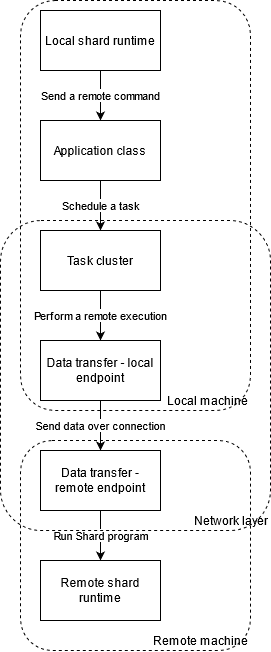
\includegraphics[scale=0.5]{img/shard_network_design.png}
    \caption{The layers of abstraction of Shard used to execute remote commands.}
    \label{fig:network_layer_design}
  \end{center}
\end{figure}

\subsection{Data transfer design}
There are four roles in the data transfer portion of the Shard network layer: the Local Sender, Local Receiver, Remote Sender, and Remote Receiver.
The name of the role describes the machine in which the role is on, and the primary direction of data flow performed by the role.
Table \ref{fig:roles_design} gives a summary of each of the four roles.

\begin{table}
  \begin{center}
    \begin{tabularx}{\textwidth}{|l|l|l|X|}
      \hline
      Role            & Location       & Connects to     & Summary                                                                                                         \\ \hline
      Local Sender    & Local machine  & Remote Receiver & Sends the data about the program to be executed, the environment, and any standard input to the remote machine.
      \\ \hline
      Remote Receiver & Remote machine & Local Sender    & Receives the data from the local sender and passes it to Shard to run the remote program.
      \\ \hline
      Remote Sender   & Remote machine & Local Receiver  & Sends the output of the remote execution back to the local machine.
      \\ \hline
      Local Receiver  & Local machine  & Remote sender   & Receives the data from the remote sender and passes it to the local Shard program as the results.
      \\ \hline
    \end{tabularx}
    \caption{The four roles involved in the Shard network layer's data transfer.}
    \label{fig:roles_design}
  \end{center}
\end{table}

The local sender and local receiver roles exist on the local machine, which is the machine of the entry point of Shard, where the code outside of the remote execution runs.
The remote sender and remote receiver roles exist on the remote machine, which is target machine where the remote program is being executed.

The two communication channels that are formed are between the local sender and remote receiver, which will be known as the local-to-remote communication channel, and between the remote sender and local receiver, which will be known as the remote-to-local communication channel.
Data sent in each of the communication channels are in the form of packets, where each packet contains all of the data being transferred.
Each packet contains an ID that corresponds to a specific instance performing a remote execution.
The choice of ID can be arbitrary, but different instances of remote execution must use unique IDs.
Packets sent from the remote sender, except for heartbeat packets, also contain a sequence number to ensure that responses are received in the order they are sent.
Heartbeat packets do not use a sequence number because it is acceptable for some of them to be dropped.
The first packet sent by the remote sender has sequence number 0, and subsequent packets have sequence number one greater than the sequence number of the previous packet.

Before remote execution can occur, the local instance of Shard must ensure that a compatible Shard instance exists on the remote machine.
If it does not already exist, Shard is responsible for copying the local Shard executable to the remote machine, before performing the remote execution.
This typically only happens the first time Shard executes a remote program on the specific remote machine on a given version of Shard.

When a remote execution begins, the local sender initializes the remote receiver and sends a header packet to the remote receiver.
The header packet contains the program to be executed remotely and a copy of the local environment, which contains information including variable and cluster assignments.
The remote receiver responds by acknowledging the Header packet.

Next, the local receiver initializes the remote sender.
At this point, all four roles have been initialized, and the remote program execution is can begin once the remote Shard runtime is ready.

The remote receiver sends the program and environment it obtained from the local sender to the remote Shard runtime to begin execution.
During this period, packets from the local sender are sent to the remote receiver, which get passed to the remote Shard runtime, and packets from the remote sender are sent to the local receiver which get passed to the local Shard runtime.
The local sender sends any standard input to the remote receiver with message packets, and the remote sender sends any standard output to the local receiver with message packets.
The remote sender also sends heartbeat packets at a regular interval to indicate that the remote process is running correctly.
When the standard input is closed, the local sender sends a close packet, and when the standard output is closed, the remote sender sends back a close packet.

Although sequence numbers and heartbeats are sent in the data transfer process, the design does not proscribe how they should be handled.
The data transfer abstraction can be utilized directly by an application class to implement its remote execution capabilities, where the packet transfer process on the local machine is controlled by the application class, or a higher-level abstraction on top of the data transfer abstraction may be used instead.

\subsection{Task cluster abstraction}

The task cluster abstraction builds on top the Shard data transfer process, by integrating the error handling mechanism to ensure reliability, and providing a higher level interface for application class implementations to use for remote execution.
The task cluster abstraction is used by both of the application classes specified in Shard's design, \texttt{single\_command} and \texttt{data\_parallel}, which take advantage of its features to ensure the reliability of the remote execution.

The task cluster maintains a set of remote targets and metadata associated with the targets, keeping the data transfer connections to these targets open as long as Shard is running.
Targets must be initialized by the task cluster before any remote computation is performed.

The task cluster uses the concept of tasks as its basic unit of remote computation.
When scheduling a task, the caller provides the following information:
\begin{itemize}
  \item The specific remote target the task should be executed on, or ``any'', indicating that the task may be executed on any initialized remote target, as selected by the task cluster;
  \item The remote program to be executed;
  \item A copy of the shell environment, to be used for the remote program;
  \item The standard input text to be sent to the remote machine.
\end{itemize}
If no specific remote target is specified, the task cluster will choose the remote target as determined by a process described in the \textbf{Remote target selection} section that follows.

Once the remote task is scheduled, the remote program associated with the task is executed on a remote machine, using the Shard network layer data transfer mechanism described in the previous section.
Each remote machine has a throttle that specifies the maximum number of tasks that can be scheduled on the machine at a time, with the throttle respecting the timeout mechanism to exit if the remote execution is taking too long.
All of the response packets sent by the remote machine are collected and ordered by their sequence number, as defined by the data transfer mechanism.
When the close packet and all packets with lower sequence numbers are received, the remote program output is assembled from the packets, the remote program execution is treated as a success.
The caller is notified of the success, with the output of the remote computation.

There are several ways for Shard to detect that an error has occurred in the remote program execution.
First, there may be an error directly reported by the data transfer mechanism.
Next, the remote Shard program may call the \texttt{exit} builtin command with a non-zero exit code, indicating a programmer-detected failure.

In addition, a failure may be detected when an execution of a remote task times out.
The two types of timeout that are considered are \textit{heartbeat timeouts} and \textit{program timeouts}.
If the task cluster does not receive a heartbeat within a certain amount of time, the task is considered a failure.
Furthermore, if the task is not completed within a much longer period of time, the task is also considered a failure.
The timeouts for the task cluster are all configurable, depending on the specific needs of the application class and expected network conditions.

The timeout failures capture the remaining ways in which a Shard remote execution can fail, because it is agnostic to the cause of failure, as long as we accept that Shard correctly determines when the remote execution succeeds.
We can be confident that at least all of the packets are transferred when Shard determines a computation is successful, because of the requirement that all packets up to and including the sequence number of the close packet are received, unless some highly improbable data corruption causes an incomplete set of packets to transform into a complete one.

In the case that the remote program does not execute successfully, the the same remote program with the same input is retried, potentially on a different machine in the cluster, depending on what the caller specified.
Even in the case of a retry, Shard still keeps the connection alive to the previous tries, using the ID of a packet to distinguish between different executions of the same remote program.
If any of the previous tries succeeds, that successful result will be used instead, and the responses for all other tries of that task are thrown away.
After a maximum number of retries as specified by the caller, the entire task will fail, and the caller will be notified.

The task cluster claims that, with high likelihood, a task scheduled to the task cluster will be successfully executed at least once on a remote machine in the cluster, and that it will correctly obtain the output of the successful computation, unless the maximum number of tries has been reached.
The specific remote machine the task executes on is guaranteed if it is specified when the task is scheduled.
Notably, the task may be completed more than once, particularly if a retry was invoked due to a timeout.
Using the task cluster abstraction means that the application class can take advantage of its error detection and retry mechanisms in order to reliably execute remote tasks, configuring the task cluster to suit the specific application class's needs.

\subsection{Remote target selection}
When the task cluster needs to select a remote target for program execution, by default, it tries to select the remote target in a principled way that tries to maximize the chance of success, based on data from previous tasks scheduled by the cluster.

Each remote target's chance of success is modeled by the beta distribution $\beta(a, b)$, parameterized by the number of successful attempts and failed attempts on that remote target, with $a$ equal to the number of successful attempts and $b$ equal to the number of failed attempts.

The beta distribution has the probability density function
$$ f(x) = x^{a-1}(1-x)^{b-1} / B(a, b), 0 < x < 1,$$
where
$$ B(a, b) = \Gamma(a)\Gamma(b) / \Gamma(a+b), $$
with $\Gamma$ being the gamma function.

The beta distribution is used because it is a useful model for predicting the chance that a future task will succeed on a remote machine.
The beta distribution has the property that given the parameters $a$ and $b$, the expected value sampled from the distribution is $a/(a+b)$, which is equal to the proportion of attempts that are successful.

A successful attempt is counted when a task successfully completes without reaching the timeout that invokes a retry.
A failed attempt is counted when a task causes a retry to be invoked.
This means that a task can correspond to any number of failed attempts, and up to one successful attempt.

When choosing a remote target for a task, the beta distribution of each machine is sampled, and the target with the maximum value is chosen.
This corresponds to choosing the remote target with the maximum likelihood of success.
Remote targets that are not yet connected to and remote targets that are at maximum capacity from throttling are excluded from this choice.

If all sampled values are below a certain threshold, or if no remote targets are available to be sampled in the first round, a second round of sampling is performed, this time between all of the remote targets, even those that are at maximum capacity, with a penalty applied to the sampled values of the remote targets at maximum capacity.
This second round of sampling is performed because, even if a remote target is at maximum capacity, it may still be preferred to be chosen compared to a remote target that has a lower likelihood of success.

There is also a small, configurable chance that the second round is bypassed, and a random remote target is selected instead.
This is to allow remote target that have previous failures to successfully execute tasks in order to raise their proportion of successes.

Once a maximum number of total attempts $m$ has been reached on each remote target, future attempts in addition to adding to $a$ or $b$ also remove a random previous attempt, so that $a+b$ does not exceed $m$.
An analogy to this is the scenario where each successful or failed attempt is added to an urn with a maximum capacity.
When the urn is full, a randomly selected attempt must be removed from the urn before adding the latest attempt.
This modification helps $a$ and $b$ more closely track recent successes and failures in long-running Shard programs, since a remote host being down for a long time would otherwise be penalized in selection once it is able to reexecute remote commands.

Depending on the application class, the beta sampling remote target selection feature can also be turned off, with random remote target selection being the fallback mechanism.
However, using this remote target selection mechanism with the beta distribution is usually a significant time-save over choosing the remote target randomly, as remote targets that result in failures are more likely to result in future failures.
The usefulness of the remote target selection mechanism will be evident later in examples in the \textbf{Reliable} section of the \textbf{Evaluation} chapter.

\section{Summary}

In this section, we describe the design of the Shard distributed framework, which is motivated by satisfying the core pillars as defined in the \textbf{Introduction} chapter.

The Shard programming language extends an the existing shell language with minimal additions to promote Shard's ease of use.
The \texttt{cluster} builtin command is used to set up clusters of remote machines in a simple fashion.
The remote execution operator extends existing shell syntax to allow Shard programs to execute sub-programs remotely on a cluster.

Application classes describe the semantics of remote execution on a cluster, and allow Shard to support a variety of use cases, with two of them described in this chapter.
The \texttt{single\_command} application class allows a Shard program to run remote commands reliably on all machines in a cluster.
The \texttt{data\_parallel} application class enables a Shard program to perform a set of remote computations on a cluster in a MapReduce-like fashion.
Although only two are mentioned in this chapter, the design of Shard supports adding more application classes as needed by additional use cases.

The network layer includes features to support performing distributed computation in a reliable manner.
The data transfer abstraction describes the steps Shard takes to set up its connections to the remote machine, with the four roles working together to transfer various types of packets.
The task cluster abstraction builds on top of the data transfer abstraction, allowing application classes to send individual tasks that will be reliably completed by the remote cluster, using a series of error handling mechanisms.
The task cluster also includes a process for choosing which remote machine to execute a program on, based on the past success rate of that remote machine.

Shard's design serves as a blueprint for its potential implementations, including an implementation described in the upcoming \textbf{Implementation} chapter.
The proof of the efficacy of Shard's design at achieving its goals is tested in the \textbf{Evaluation} chapter that appears later in this thesis.


\chapter{Implementation}

In this chapter, we discuss the implementation of Shard, which includes the implementation of the shell, the language, the protocol, and the application classes.

\section{Overview}

Shard is implemented in the OCaml programming language, as a single project that includes the shell, language, network layer, and application class components of Shard, along with code that combines these components into a single application.
OCaml was chosen for its convenience in programming language implementation, high level of safety, direct access to UNIX system calls with a wrapper library, reasonable performance, and programmer familiarity of the language.

When built, Shard is an executable invocable on the command-line that can be used in a similar fashion as other executable shell programs, by passing it a file containing a shard program (typically with the \texttt{.shard} extension), or by passing in no arguments to start Shard in interactive mode.
Interactive mode allows Shard to function as a Read-Eval-Print-Loop, meaning that the user can input any Shard command followed by an \texttt{Enter} key press to execute it, giving back control to the user when the command execution completes.
Like for some other shells, Shard allows the user to use the keyboard shortcut \texttt{Ctrl-C} to interrupt the current executing Shard command, and the keyboard shortcut \texttt{Ctrl-\textbackslash} to immediately exit Shard.
% Specific usage details can be found in the documentation of the project.

Currently, Shard is specifically tested to support Ubuntu Linux version 20.04.2 LTS, but it likely works with few modifications on other UNIX systems, depending on the requirements of the library dependencies of Shard.

\section{Architecture}

% \begin{itemize}
%   \item Split up into 4 parts: Shell, language, network layer, application class
%   \item Basic summary of each part, its purpose, and how they connect together
% \end{itemize}

The Shard project is split up into four parts: shell, language, network layer, and application classes. The split is conceptual, as all four parts belong to the same compilation unit, and reside in the same directory.
Each of the sections of the architecture are designed in a way to be easily extensible, in that more functionality can be added without significantly changes to existing code.

The shell is connects the program and the interactive mode to the remaining parts of Shard. This is also the entry point of a Shard program.

The language provides the Shard programming language features, including a recursive descent parser and a tree-walk interpreter. The interpreter also communicates with the network layer and the application classes as needed by the command that it is currently executing, in addition to the operating system for a variety of shell features.

The network layer provides all of the distributed systems functionality, including maintaining network connections to remote machines, spawning helper processes, and error detection/handling.

\begin{sloppypar}
  The application class includes the interfaces of the application class subsystem and the implementation of the specific application classes that are currently supported, which are the \texttt{single\_command} and \texttt{data\_parallel} application classes. Application classes are described in more detail in the \textbf{Application Classes} section of the \textbf{Design} chapter.
\end{sloppypar}

% \todoi{Future: Simple figure for architecture}

In addition to these specific parts of Shard, there are also modules for common utility functions, unit testing, and command-line interfacing.

\subsection{Dependencies}
The Shard project depends on various other OCaml libraries and OCaml wrappers for non-OCaml libraries for important pieces of existing functionality.

The entire project is written on top of Jane Street's open source libraries Core, Async, and Sexplib, along with the OCaml parser combinator library Angstrom and an OCaml wrapper for the SSH library \texttt{libssh}.

Core is an alternative standard library for OCaml with many more features, including additional data structures and extensions to existing standard library modules \cite{ocamlcore}.
Core also provides full UNIX support in its \texttt{Core.Unix} module, including API wrappers for many of the system calls found in Linux and other UNIX machines.

Core depends on the Jane Street library Sexplib, which contains functionality for working with S-expressions, a human readable data representation format commonly used by the LISP family of languages \cite{mccarthy1960recursive}. Sexplib allows automatic generation of functions to convert OCaml objects to and from S-expressions, and is used extensively to convert objects for serialization purposes.

Async provides promise-based asynchronous code support for OCaml, and includes its own \texttt{Async.Unix} that builds on top of \texttt{Core.Unix} to allow system calls and I/O operations to work asynchronously on top of an event queue, while still working under the OCaml language's single core restriction \cite{ocamlasync}.

Shard's language parser depends on the OCaml parser combinator library Angstrom, which is designed to be an easy-to-use parser combinator library specifically for use with OCaml. \cite{ocamlangstrom}.
Shard uses a forked version of Angstrom that adds a few more combinators to Angstrom's long list in order to support specific features of the shell grammar that would otherwise be more difficult to implement with Angstrom's existing interface.

Shard's network layer depends on the SSH library \texttt{libssh} for all of its network communication \cite{libssh}.
\texttt{libssh} is a widely used SSH library implemented in C that includes compatibility with all of the SSH communication features needed by Shard.
Because \texttt{libssh} is written in C, Shard uses a publicly available open source OCaml wrapper for \texttt{libssh}, \texttt{mllibssh} \cite{mllibssh}.
Due to issues with \texttt{mllibssh} not being well maintained, the version of \texttt{mllibssh} used in Shard is forked and contains modifications including bugfixes and improvements to the wrapper code.


\section{Shell implementation}

% \begin{itemize}
%   \item In depth writing about how the shell is implemented
%   \item OCaml, directly on top of Unix primitives (rather than on an existing shell)
%   \item Invokable with command-line
%   \item Interactive and non-interactive mode
%   \item Most features are written to work locally, and separated so that language/network layer/application class implementations are abstracted
% \end{itemize}

The Shard shell is implemented in OCaml, directly on top of UNIX primitives from the OCaml libraries Core and Async.
An alternative solution would be to take an existing shell application and modify it to support the Shard programming language and platform, which would have the benefit of letting Shard support many additional shell features for free, such as tab-completion, history, and custom colors, depending on the feature set of the shell it extended.
However, using an existing shell would also offer much less flexibility in terms of making changes that radically transform the behavior of the shell, such as making remote execution functionality seamlessly work alongside local functions in the shell.

When the shell is invoked in interactive mode, it works as a Read-Eval-Print-Loop (REPL). The REPL reads a line from the standard input (stdin) for a Shard command or program. The shell sends the input to the parser, which results in either an abstract syntax tree (AST) corresponding to the input, an error in parsing, or an incomplete parse.
In the case of a successful parse of an AST, the resulting AST is evaluated by the interpreter, and any output of the command is forwarded to the standard output (stdout) or standard error (stderr), before returning to REPL to wait for the input of a a new command.
In the case of the incomplete parse, another line is read from standard input and added to the original input to try parsing again.
In the case of a parse error, the error is printed back to the standard error (stderr), and the REPL waits for further input for a new command.
The text below showcases an example of the output when running Shard interactively:

\begin{minipage}[c]{\textwidth-15pt}
  \begin{lstlisting}[language=Shard]
$ echo "Hello, world!"
Hello, world!
$ (cat /etc/issue)@@machine1
Ubuntu 20.04.2 LTS \n \l

$
\end{lstlisting}
  \smallskip
\end{minipage}

Similarly, when the shell is invoked in non-interactive mode, the shell sends the input file or string to the parser, which results in either an AST corresponding to the input program, or an error if the input fails to parse, in which case the error is printed to stderr.

The shell can be invoked with the \texttt{-s} command-line flag to indicate that the input is an S-expression that represents an AST object rather than a string in the Shard language grammar. In this case, the step of parsing with an AST is bypassed, and the AST is directly evaluated by the interpreter, behaving identically to if it were parsed from a program in the language.
This is useful when using Shard to execute programs that have previously been parsed, such as when the Shard runtime wants to run a Shard program on a remote machine.

The shell also uses the concept of jobs control support the keyboard interrupt feature, which allows the user to cancel the currently running task.
Shard uses a signal handler to catch the \texttt{SIGINT} interrupt signal when \texttt{Ctrl-C} is pressed during a running task.
Rather than exiting Shard itself, instead this causes the Shard evaluation to stop, as each evaluation function checks to make sure that the job is active before performing the evaluation.
If an external command is currently being executed, the signal is passed to that command. If a remote command is currently being executed, further progress is stopped by sending a message over the data transfer layer.

\section{Language implementation}

% \begin{itemize}
%   \item Implemented by referring to POSIX shell specification
%   \item Parse: Use recursive parser combinator library Angstrom
%   \item Interpret: Interpret parsed objects in functions directly, with support for custom features needed by Shard
%   \item Some specification features are not yet supported, but there is no reason why support cannot be added if needed
% \end{itemize}

The Shard programming language implementation is split up into two main parts -- the recursive descent parser and the tree-walk interpreter.

\subsection{Shard parser}

The parser is implemented using the parser combinator library Angstrom by following the grammar section in the POSIX shell specification, and extending it with the additional syntax found in the \textbf{Language design} section of the \textbf{Design} chapter \cite{ocamlangstrom} \cite{posix2017}.

The OCaml variant type can be used very effectively to represent recursive structures with complex definitions, along with retrieving their data in a type-safe manner using pattern matching, which is one of the significant benefits to using OCaml for implementing programming languages \cite{realworldocaml}.

A successful parse transforms a \texttt{string} input to a \texttt{Ast.t} variant as output. The \texttt{Ast.t} variant is used to represent a Shard abstract syntax tree, which is also used in the interpreter when walking through the AST.

In addition to allowing the parsing of full strings that are defined by the Shard grammar, the parser also uses an Angstrom feature to support partial parsing, which uses a piece of state to describe whether a parse is complete (the input is a string in the grammar), incomplete (there exists some string that completes parse), or failed (there is no string that completes the parse).
This allows the user to enter a new line after partially inputting their command in the interactive shell, and have the shell prompt for more input, rather than rejecting the input.
Note that inputting an empty line will force the parse to attempt to complete, which will in this case indicate that the parse failed.

For example, inputting the Shard command gives a prompt of \texttt{>} to continue with the command, as the parser sees the unmatched open parentheses.

\begin{minipage}[c]{\textwidth-15pt}
  \begin{lstlisting}[language=shard]
$ (echo
>
\end{lstlisting}
  \smallskip
\end{minipage}

This command can be completed by adding some input and closing the parentheses.

\begin{minipage}[c]{\textwidth-15pt}
  \begin{lstlisting}[language=shard]
$ (echo
>  hello)
hello
$
\end{lstlisting}
  \smallskip
\end{minipage}

One notable distinction between Shard and other shell parsers is that nested shell environments such as subshells in Shard are parsed together with the entire command, rather than as needed.
In the Bash shell, for example, if a subshell is defined in a branch of a boolean expression, and there is a syntax error in the subshell, the result would only be a syntax error if the branch gets evaluated.
On the other hand, in Shard, the parser would fail to parse the entire expression due to failing to parse the subshell.

As such, the following shell program would result in a syntax error in Shard, but not in Bash, because the right-hand-side of the boolean expression is never evaluated in Bash:

\begin{minipage}[c]{\textwidth-15pt}
  \begin{lstlisting}[language=shard]
false && $(|)
\end{lstlisting}
  \smallskip
\end{minipage}

The parser's interface exposes the functions that are called by the other parts of the program to convert between Shard programs as strings to its AST. The following OCaml interface describes the input and output types of the parser:

\begin{minipage}[c]{\textwidth-15pt}
  \begin{lstlisting}
(* Excerpt from ast.mli *)
(* AST type definition omitted *)
type t
(* ... *)
[@@deriving sexp]

val parse : string -> t Or_error.t

val parse_partial
  :  ?state:t Angstrom_extended.Buffered.state
  -> string
  -> t Angstrom_extended.Buffered.state
\end{lstlisting}
  \smallskip
\end{minipage}

As we can see from this interface, the \texttt{parse} function performs a regular parse of any input string, and emits an \texttt{Ast.t Or\_error.t} variant, which either holds the value of an \texttt{Ast.t} variant (the representation of the AST itself), indicating a successful parse, or an \texttt{Error.t} record, indicating a failed one.

In addition to the \texttt{parse} function, the interface also exposes the \texttt{parse\_partial} function. This corresponds to the partial parsing behavior as described above, taking in an optional partial parsing state and the input string, and spitting out a new partial parsing state corresponding to the status of the partial parse.

Furthermore, from the definition of \texttt{Ast.t}, we can see that it includes the OCaml preprocessing instruction \texttt{[@@deriving sexp]}. This autogenerates functions that allow conversion of the \texttt{Ast.t} variant to and from the \texttt{Sexp.t} variant, which represents an S-expression that losslessly encodes the AST and can be transmitted as a string.

\subsection{Shard interpreter}

The Shard interpreter is a tree-walk interpreter that crawls through the abstract syntax tree and evaluates it node-by-node.
The interpreter is implemented with a set of mutually recursive functions, with each function taking the name \texttt{eval\_PART}, where \texttt{PART} indicates the node on the AST being evaluated by that function.
Evaluating an AST node involves calling the \texttt{eval\_PART} functions corresponding to its children nodes, if any, and then performing an operation based on the type of node being evaluated.

% A concrete example of a type of branch node of the AST is the type \texttt{Ast.pipeline}, with the following definition
% \begin{lstlisting}
% type t = (* ... *)
% and pipeline = bang option * command list
% and bang = Bang
% \end{lstlisting}

% The pipeline represents a chain of commands piped together in Shard, where the entire pipeline can be optionally negated by a bang (\texttt{!}) symbol to change the truthiness of its return code.
% Here is a shell program that finds all of the lines of the input with the character `!':
% \begin{lstlisting}[language=shard]

% cat input.txt | grep "!"

% \end{lstlisting}

% This is represented by a \texttt{Ast.pipeline} made up of the \texttt{None} option}, followed by two \texttt{Ast.command}s.

% The following excerpt from the \texttt{eval\_pipeline} function demonstrates evaluating an \texttt{Ast.pipeline}:

% \begin{lstlisting}
% (* Excerpt from eval.ml *)
% and eval_pipeline pipeline ~eval_args =
%   match pipeline with
%   | [] -> return 0
%   | x :: xs ->
%     (match xs with
%     | [] -> eval_pipeline_part x ~eval_args
%     | _ ->
%       let pipe_read, pipe_write = Pipe_process.pipe () in
%       let deferred_code =
%         eval_pipeline_part x ~eval_args:{ eval_args with Eval_args.stdout = pipe_write }
%       in
%       let new_deferred_code =
%         eval_pipeline xs ~eval_args:{ eval_args with Eval_args.stdin = pipe_read }
%       in
%       let%bind _code = deferred_code in
%       let%bind () = Fd.close pipe_write in
%       let%bind new_code = new_deferred_code in
%       let%bind () = Fd.close pipe_read in
%       return new_code)
% \end{lstlisting}

% Most AST nodes behave as they would in other shell languages, and their implementation is based on following the semantics as defined by the POSIX specification.
% Some notable examples of AST nodes that are treated differently in Shard are \texttt{Ast.subshell} and \texttt{Ast.remote\_command}.

The basic building block of the shell is the simple command, made up of a command name and command arguments, along with any assignments and I/O redirections that are associated with the command.
The command name can either refer to a builtin or an external command.
In the case of a builtin, the functionality is implemented in OCaml itself as a part of \texttt{builtin.ml}.
In the case of an external command, it is executed using the Spawn library, a dependency of the OCaml Core library, behaving in a similar manner to the \texttt{exec} system call, taking in as input the command name, arguments, environment, and associated file descriptors for the standard I/O.

During evaluation, a record of the type \texttt{Eval.Eval\_args.t} is passed to each \texttt{eval\_PART} function to represent the input state required for the evaluation to succeed. The definition of the record is shown below:

\begin{minipage}[c]{\textwidth-15pt}
  \begin{lstlisting}
(* Excerpt from eval.ml *)
module Eval_args = struct
  type t =
    { env : Cluster_type.t Env.t
    ; stdin : Fd.t
    ; stdout : Fd.t
    ; stderr : Fd.t
    ; verbose : bool
    }
  [@@deriving fields]
  (* some function definitions omitted *)
end
\end{lstlisting}
  \smallskip
\end{minipage}

The \texttt{Eval\_args.t} is made up of the shell environment (\texttt{Cluster\_type.t Env.t}), file descriptors for the standard I/O of the command being evaluated, and a verbose flag.
By default, the standard I/O corresponds to the standard I/O of the Shard program itself.
This is modified when pipelining and I/O redirecting are introduced.

A pipeline indicates that the output of a command should be passed to the input of the next command with a pipe, as shown in the following example shell program that finds all of the lines of the input with the character `!':

\begin{minipage}[c]{\textwidth-15pt}
  \begin{lstlisting}[language=shard]
cat input.txt | grep "!"
\end{lstlisting}
  \smallskip
\end{minipage}

Originally, this was achieved by manually transferring the data from one program to the next with a virtual pipe-like construct, but this resulted in many practical problems, such as producing the correct behavior when the pipe is closed on either end.

Thus, the piping behavior was changed to use UNIX pipes.
When a pipe operation occurs, a UNIX pipe is created.
The environment's stdin is used as the first command's stdin file descriptor, the environment's stdout is used as the second command's stdout file descriptor, and the two ends of the UNIX pipe are used as the remaining two file descriptors to join the first command's output with the second command's input.
This can be invoked recursively to easily extend support arbitrarily to many commands in a pipeline.
When both programs exit, the pipe must be explicitly closed.
Otherwise, a resource leak can occur, where the Shard runtime stops functioning due to reaching a limit on the number of open file descriptors.
When this data is piped to a remote program, the way the data is handled depends on the application class of the remote cluster.
For example, the \texttt{single\_command} application class passes the piped input to the standard input of each of the remote programs that is being executed.

File I/O redirection works in a similar manner to pipelining, setting a stdio file descriptor to a file with the specified filename.
Currently, the Shard interpreter does not support I/O redirection on custom file descriptors other than the standard I/O, but the \texttt{Eval\_args} can be augmented to support the additional redirection capabilities as needed.

A defining feature of Shard is its remote command execution capabilities, where an example of a remote command is shown in the following example that prints out the operating system version of a remote machine:

\begin{minipage}[c]{\textwidth-15pt}
  \begin{lstlisting}[language=shard]
$ (cat /etc/issue)@@machine1.cs.williams.edu
Ubuntu 20.04.2 LTS \n \l

$
\end{lstlisting}
  \smallskip
\end{minipage}

Evaluating a remote command is implemented in a similar fashion to evaluating a subshell.
However, for remote execution, all of the pieces of information needed to evaluate the expression are serialized into S-expression form and sent across the network to a remote instance of the Shard runtime.

If the target of the remote command is a cluster, the application class implementation associated with the cluster will be used for specifics on the execution of the remote command.
% which exposes the following public API to the interpreter:
% \begin{lstlisting}
% (* Excerpt from application_class.ml *)
% val remote_run
%   :  cluster_id:string
%   -> remote_targets:Remote_target.t list
%   -> setting:string
%   -> program:Sexp.t
%   -> env_image:Env_image.t
%   -> verbose:bool
%   -> stdin:Reader.t
%   -> stdout:Writer.t
%   -> stderr:Writer.t
%   -> unit Deferred.Or_error.t
% \end{lstlisting}
On the other hand, if the target is a host (which is assumed to be the case when the cluster with the given name is not found), the default application class implementation behaving similarly to the \texttt{single\_command} application class is used instead.
More details of the remote execution will be specified in the \textbf{Network layer implementation} section.

% \todoi{Future: Maybe include a section on asynchronous execution (shell ampersand operator)}

As of the time of writing, some of the features in the POSIX shell specification are not supported by the parser or interpreter of the Shard shell.
However, there is no reason why support for these features cannot be added if needed.
We focused on implementing the most commonly used features, with the primary constraint being that the POSIX shell specification is extremely long and contains many features that are not very commonly used by most users in practice.

\section{Network layer implementation}

% \begin{itemize}
%   \item Model: copy executable to each remote machine, then use SSH to communicate between machines
%   \item Support SSH config
%   \item Each remote invocation spawns two processes locally and two processes remotely: justified by easy to separate remote invocations
%   \item Use OCaml Async RPC for interprocess communication between processes on the same machine: strongly typed, serialization supported, etc
%   \item Heavyweight but works well for ad hoc programming
% \end{itemize}

Many choices can be made in terms of deciding on how to implement the network layer of Shard.
The choices outlined in this section are chosen based on a variety of criteria, including availability, usability, and ease of implementation.

\subsection{Network transport}
Our implementation uses the Secure Shell (SSH) protocol as a basis for data transportation and communication over the network.
SSH is a widely supported protocol for accessing a command-line shell on a remote machine over a network (usually on top of TCP), with the popular implementation OpenSSH available on many UNIX platforms \cite{openssh}.
SSH supports security, authentication, and privacy, so those features are leveraged by Shard and do not have to be built into our implementation from scratch \cite{rfc4251}.

Shard uses the SSH library libssh by leveraging its implementation of the SSH client protocol.
Currently, authentication is handled by using SSH key-pairs to automatically perform authentication.
For each remote machine in the cluster, the local user should have set up key-based SSH access through OpenSSH by adding the local user's public key to the \texttt{authorized\_keys} of the remote host.
If the user has an OpenSSH configuration file (\texttt{sshd\_config}) at the default location (at \texttt{~/.ssh/}), it is used to allow custom host names and private key names, which can be used for remote targets in the cluster definition.
Otherwise, the user should make sure that the necessary keys are added to their OpenSSH agent for automatic authentication.
This authentication procedure is standard for regular SSH access, and Shard does not need anything extra in order for the SSH transport to work correctly.

\subsection{Data transfer framework}

The Shard network layer sets up two connections between two pairs of endpoints in order to perform all of the necessary data transfers.
This is implemented by running four additional instances of Shard whenever a remote command is executed on a remote host, each in a separate process.
Separate processes are used for each instance specifically to make it easier to support many simultaneous remote connections while being able to recover from failures by killing processes and spinning up new ones as needed.
Subsequent remote commands on the same remote host attempt to reuse the same four instances of Shard, as creating new instances is a relatively expensive operation.

These four instances each correspond to a role as specified by the design of the Shard network layer, as specified in the \textbf{Data transfer design} section of the \textbf{Design} chapter.
The four roles are Local Sender, Local Receiver, Remote Sender, and Remote Receiver, with the two local processes being on the local machine, and the two remote processes being on the remote machine.
The procedure for executing a remote command is shown in Figure \ref{fig:network_layer_impl}, and will be explained in more detail in the \textbf{Data transfer setup} and \textbf{Remote program execution flow} sections that follow.

\begin{figure}[h]
  \begin{center}
    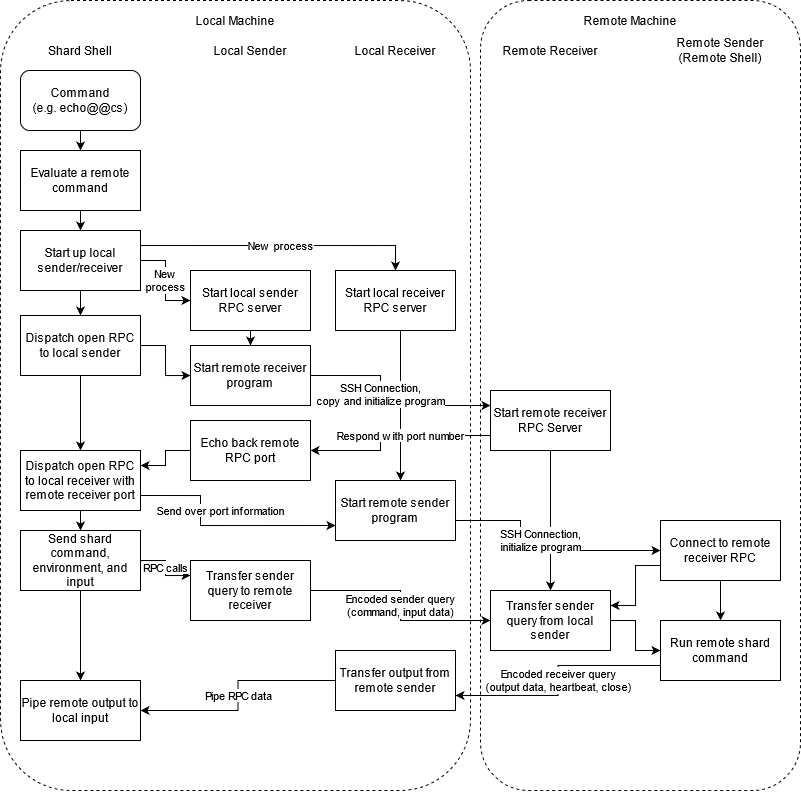
\includegraphics[scale=0.49]{img/shard_protocol_impl.png}
    \caption{The procedure for executing a remote command with the Shard network layer.}
    \label{fig:network_layer_impl}
  \end{center}
\end{figure}

The processes on the same machine communicate with each other using remote procedure calls (RPC) from the RPC library Async\_rpc, which is a part of the OCaml Async library.
This library allows the creation of type-safe RPCs that automatically serialize queries and responses with the help of OCaml annotations, making it very easy to set up an RPC service for all of the remote calling functionality necessary.
The RPC servers are accessed by invoking an RPC dispatch call on a particular port on the machine, which is randomly generated and given to the program when the RPC server is created.
Although the RPC servers are not particularly lightweight, only two are used on the local machine for each remote machine connection, so this does not cause a usability problem from a performance standpoint.

\subsection{Data transfer setup}

As mentioned earlier, all of the data transfer and communication setup is coordinated over SSH, which runs on top of TCP.
The first step of the setup is making a copy of the local Shard executable on which to run the Local Sender and Local Receiver.
Note that all four processes use an identical executable to the original Shard executable, but with a command-line argument indicating which role the processes takes on, as described in Table \ref{fig:process_role_args}.
These command-line arguments should only be used internally by the remote execution mechanism for Shard, and not used by the end user.

\begin{table}[h]
  \begin{center}
    \begin{tabular}{|l|l|l|l|}
      \hline
      Process role    & Connects to     & Argument & Additional arguments               \\ \hline
      Local Sender    & Remote Receiver & -Rls     &                                    \\ \hline
      Local Receiver  & Remote Sender   & -Rlr     &                                    \\ \hline
      Remote Sender   & Local Receiver  & -Rrs     & Port of Remote Receiver RPC server \\ \hline
      Remote Receiver & Local Sender    & -Rrr     &                                    \\ \hline
    \end{tabular}
    \caption{The command-line arguments for running the executable as each of the four roles in Shard's data transfer.}
    \label{fig:process_role_args}
  \end{center}
\end{table}


The local copy of Shard is made with a \textit{copy attempt}, with the source being the currently running executable, and the destination being a directory known as the Shard cache, using a fixed path.
A copy attempt includes checking whether a Shard executable exists at the destination location, and comparing a cryptographic hash value of the destination file's contents with the source file to make sure that if the file exists, it is the exact same version.
If either no file exists or the destination file has a different hash from the source file, a copy is made.
The reason to make a copy attempt rather than to always make a copy is to save the network resources used to perform such a copy when possible.

Once the local copy of Shard is successfully created, the Local Sender and Local Receiver processes are spawned.
Upon spawning, RPC servers are created for the Local Sender and Local Receiver, and their ports are printed to standard output so the parent processes is able to make dispatch RPC calls to the two processes.

The second step that the Shard network layer performs is to distribute a copy of the Shard executable to the remote machine, using the same copy attempt mechanism previously mentioned.
This is done by dispatching an \texttt{Open} RPC query to the Local Sender, which has the following record type as its query type:

\begin{minipage}[c]{\textwidth-15pt}
  \begin{lstlisting}
(* Excerpt from rpc_local_sender.ml *)
module Open_query = struct
  type t =
    { host : string
    ; port : int option
    }
  [@@deriving bin_io, fields]
end
\end{lstlisting}
  \smallskip
\end{minipage}

The annotation \texttt{[@@deriving]} indicates that the compiler will autogenerate code for the record type, where \texttt{[@@deriving bin\_io]} autogenerates functions to serialize the record in binary form for the RPC, and \texttt{[@@deriving fields]} autogenerates getter functions for accessing individual fields.
For this query, the Local Sender uses the SSH shell copy (SCP) functionality to make a copy attempt of the Shard executable to the remote machine.
In this case, it is particularly important to check if the Shard executable already exists in the remote Shard cache, as transferring the executable every time can be very expensive in terms of bandwidth and time.

Once the Shard executable is copied to the remote machine, the next step is to spawn the Remote Receiver processes on the remote machine from the Local Sender via SSH's shell execution mechanism.
The Remote Receiver also creates and RPC server that is used to communicate with the Remote Sender at a later point.
This Remote Receiver RPC server's port is passed back to the Local Sender, and then passed back to the parent process as the query response to the \texttt{Open} query.

Next, the Local Receiver spawns the Remote Receiver sender processes on the remote machine, once again via SSH's shell execution mechanism, and passes in the port of the Remote Receiver RPC server, allowing the Remote Receiver to be connected to the Remote Sender with a pipe on top of the RPC service.

Finally, the system is ready to accept a remote program execution.
Note that future remote program executions on the same remote host can reuse the same four processes, so the earlier steps are only necessary when starting a remote program execution on a new host, or if the processes fail and re-execution is scheduled on a new set of processes.

\subsection{Remote program execution flow}

When a remote program is executed, the first step involves dispatching a \texttt{Header} RPC to the Local Sender, which has the following record type as its query type:

\begin{minipage}[c]{\textwidth-15pt}
  \begin{lstlisting}
(* Excerpt from rpc_common.ml *)
module Header = struct
  type t =
    { program : Sexp.t
    ; env_image : Env.Image.t
    }
  [@@deriving sexp, bin_io, fields]
end
\end{lstlisting}
  \smallskip
\end{minipage}

% \todoi{Future: AST representation S-expression example }

As shown here, the query for starting the remote program includes the program's AST representation \texttt{Ast.t} in S-expression form, as a \texttt{Sexp.t}, and a serializable image of the environment \texttt{Env.t}, which includes parts of the shell execution environment for this specific program's execution, such as assignments and cluster definitions.
In addition to the \texttt{[@@deriving bin\_io]} and \texttt{[@@deriving fields]} mentioned in the previous section, this record type also contains the \texttt{[@@deriving sexp]} annotation to autogenerate functions for serialzing and deserializing the record as an S-expression, which is useful when sending the query as an S-expression string over SSH.
% reasoning for remote sender/receiver will be explained in the design section
The Local Sender uses SSH to send the entire query in S-expression form to the Remote Receiver, which passes the query on to the Remote Sender.
The Remote Sender Shard process is the one that actually performs the program execution, using the program and environment as specified by the query.
In addition to the \texttt{Header.t} query, the Local Sender also generates a unique ID for this program execution that is sent to the Remote Receiver, which passes it along to the Remote Sender.
This ID helps keep track of the responses from the Remote Sender, as the Remote Sender may be running more than one remote program execution simultaneously, and the output from these programs may be interlaced.

The output of the execution on the Remote Sender is sent over the SSH stream back to the Local Receiver with records of the \texttt{Receiver\_query} type serialized to S-expression form:

\begin{minipage}[c]{\textwidth-15pt}
  \begin{lstlisting}
(* Excerpt from rpc_common.ml *)
module Receiver_data = struct
  type t =
    | Message of string
    | Close
    | Heartbeat of int
  [@@deriving sexp, bin_io]
end

module Receiver_query = struct
  type t =
    { id : string
    ; sequence_number : int
    ; data : Receiver_data.t
    }
  [@@deriving sexp, bin_io, fields]
end
\end{lstlisting}
  \smallskip
\end{minipage}

A \texttt{Receiver\_query} record contains a \texttt{data} field of the \texttt{Receiver\_data} variant type, in addition to the ID of the program execution and a sequence number.
The \texttt{Receiver\_data} variant shows the three types of data that can be delivered by the Remote Sender: a message for the standard output, a close notification indicating that execution is complete, and a heartbeat to indicate that the connection is still alive.
When the Local Receiver gets the \texttt{Receiver\_query} record, it uses the RPC server to send this record back to the parent process.

In addition to sending the program to be executed, the Local Sender is also responsible for sending standard input to the remote program, and notifying the remote program when the sender closes the writer writing to the standard input.
The sender query type looks very similar to the receiver query type, except that the Local Sender has no control over the heartbeat and sequence number fields of receiver query, as they originate from the Remote Sender.

\subsection{Heartbeat and sequence number handling}

The Shard network layer exposes an interface for manually processing the \texttt{Receiver\_query} records from the Remote Sender.
This allows for greater control over handling the specific pieces of functionality as provided by the network layer, such as the heartbeat, id, and sequence number. However, most users of the protocol can opt to use the \texttt{task\_cluster} interface that automatically handles reliablility and retries using these features:

\begin{minipage}[c]{\textwidth-15pt}
  \begin{lstlisting}
(* Excerpt from task_cluster.mli *)
type t

val create : unit -> t

val init_targets
  :  t
  -> targets:Remote_target.t list
  -> stderr:Writer.t
  -> verbose:bool
  -> unit Deferred.Or_error.t

val run_task
  :  t
  -> target:[ `Any | `Specific of Remote_target.t ]
  -> program:Sexp.t
  -> env_image:Env_image.t
  -> send_lines:string list
  -> string Deferred.Or_error.t
\end{lstlisting}
  \smallskip
\end{minipage}

The \texttt{task\_cluster} interface exposes the abstraction of tasks that need to be completed on a cluster.
When a \texttt{task\_cluster} is created, the set of possible remote targets need to be initialized with \texttt{init\_targets}, which performs the data transfer setup of getting the remote machine ready for accepting remote commands on each remote target passed in.

When a task is created with \texttt{run\_task}, it is executed on an arbitrary or specific target, depending on what is desired by the caller.
If the arbitrary target is selected, a beta sampler is used to choose the remote machine with the maximum likelihood of success, following the selection process as described in the \textbf{Remote target selection} section of the \textbf{Design} chapter.
Successful and failed remote execution attempts are recorded by the beta sampler, which help future remote task executions prioritize remote machines that are more likely to succeed.

\begin{sloppypar}
  All of the information of the program execution is contained in the \texttt{program}, \texttt{env\_image}, and \texttt{send\_lines} parameters, the first two of which are sent as a \texttt{Header.t} record to start the remote computation. The third parameter is the lines provided to the standard input of the program.
  This task is created with a timeout mechanism that will cause the task to be retried, based on various conditions: if the first heartbeat is not received after a set amount of time; if further heartbeats are not received after some time; or if the entire processes's execution takes too long.
  A retry is also invoked if an error occurs during the task's execution.
  In this case, a further error recovery mechanism is used to reinitialize the remote target with a new set of processes, which allows the task to recover from Shard crashes.
  This retry mechanism can result in the same task being executed multiple times on different machines, until the task comes back with a successful result (a close message).
\end{sloppypar}

In addition, the \texttt{task\_cluster} keeps track of the sequence number of the \texttt{Receiver\_query}s being sent by the Remote Sender, to make sure the queries are processed in the correct order.
It does so by keeping track of the highest sequence number currently seen, storing messages out of sequence in a hash table until they are the next message in sequence, and producing the final output string when the close query is received.
This means that no output is lost, even if the close query reaches the local machine before some standard output message sent earlier by the Remote Sender.
If a query is dropped, the close query will never be in sequence, so the timeout mechanism will time out the execution, and a retry will be invoked.

Using the \texttt{task\_cluster} abstraction, the caller can be confident that tasks will be continously reattempted until it completes successfully (or wait forever if the task always fails).
Even though the many levels of abstraction used result in a more heavyweight network layer, it is a worthwhile trade-off to ensure that Shard satisfies the core pillars of being reliable and easy to use. It also works well enough for running ad hoc programs that do not utilize all system resources.

\section{Application class implementation}

% \begin{itemize}
%   \item Each application class implementation conforms to a specific interface
%   \item Handles how new jobs are dispatched, how existing jobs are managed, retry, error handling, etc. as needed by the application class
%   \item Ability to plug in support for new application classes
% \end{itemize}

Application classes are implemented in the Shard project as instances of an application class module type, which specifies the following interface:

\begin{minipage}[c]{\textwidth-15pt}
  \begin{lstlisting}
(* Excerpt from application_class.ml *)
module type Backend = sig
  val remote_run
    :  cluster_id:string
    -> remote_targets:Remote_target.t list
    -> setting:string
    -> program:Sexp.t
    -> env_image:Env_image.t
    -> verbose:bool
    -> stdin:Reader.t
    -> stdout:Writer.t
    -> stderr:Writer.t
    -> unit Deferred.Or_error.t
end
\end{lstlisting}
  \smallskip
\end{minipage}

This function is called by the Shard evaluator's remote execution evaluation, which supplies the application class with each of the parameters of the \texttt{remote\_run} function as necessary to successfully perform the remote execution.
The implementation of this function depends on the specific application class backend, but generally involves calling functions in one of the remote invocation abstractions provided by the Shard network layer implementation, which then performs the actual remote program execution.
Repeated remote execution calls on the same cluster are guaranteed to use the same \texttt{cluster\_id} string, meaning that the backend can partition its inputs on a per-cluster basis, using global state to maintain a lookup for individual cluster data from its ID.

Although there are currently only two application classes implemented in Shard, it is easy to create additional ones by creating modules that follow the specification of the module type, which contains all of the information needed by the application class to support any unique features.
Currently, the project's source code needs to be modified to add builtin support for the application class. However, with some minor changes, it would be possible to externally expose all of the controls for which application classes to use, meaning that Shard could be used as a library on which to build additional remote capabilities on top.

\subsection{Single command}

\begin{sloppypar}
  The \texttt{single\_command} application class supports functionality for running a command that will be reliably executed on each of the machines in a cluster in a best-effort manner. The following example \texttt{single\_command} program gets the system information of all machines in a cluster named \texttt{csmachines}, and prints it to the local output:
\end{sloppypar}

\begin{minipage}[c]{\textwidth-15pt}
  \begin{lstlisting}
(uname -a)@@csmachines 
\end{lstlisting}
  \smallskip
\end{minipage}

\begin{sloppypar}
  The implementation of this application class is very simple, and does not require directly using the Shard network layer's RPC queries: it takes the program input, and uses the \texttt{task\_cluster} abstraction to reliabily execute the program as a task on each machine in the cluster.
  The \texttt{task\_cluster} guarantees reliability and error recovery, allowing the task to be retried on the same machine if it fails.
\end{sloppypar}

\subsection{Data parallel}

The \texttt{data\_parallel} application class supports MapReduce-style functionality for running intensive multi-phased data-parallel applications.
The following example \texttt{data\_parallel} program calculates the number of occurrences of each line length in an input file on the cluster named \texttt{testcluster}, which has already been defined and set to be using the \texttt{data\_parallel} application class:

\begin{minipage}[c]{\textwidth-15pt}
  \begin{lstlisting}[language=shard]
cat input.txt |
    (echo $in | wc -c; echo 1)@@map/testcluster |
    (paste -sd+ - | bc)@@reduce/testcluster
\end{lstlisting}
  \smallskip
\end{minipage}

When the \texttt{data\_parallel} application class backend receives the \texttt{remote\_run} call, it gets two separate calls, one with the ``map'' setting and one with the ``reduce'' setting.
The backend's functionality is based on the setting of the call, and fails if the setting is not either ``map'' or ``reduce'', as these are required by the \texttt{data\_parallel} application class backend.

For the call with the ``map'' setting, the backend splits the input by line, and creates a task for each line, where the task is to execute the remote execution payload specified by the \texttt{program} argument.
The environment for this execution is a copy of the local environment with an additional assignment of the variable \texttt{\$in} to the value of the line.
This is sent to an arbitrary remote host for execution, chosen by the \texttt{task\_cluster} abstraction provided by the network layer, which also ensures that the task is reliably completed.
The program is expected to output two lines: the first of which is the key, and the second of which is the value.
This is printed to the local standardout as a key-value pair in a single line, with the key and value separated by a comma.

For the call with the ``reduce'' setting, it expects the input to be in the form of the ``map'' output, where each input's line is a key-value pair separated by a comma.
The backend aggregates the inputs by key, and sends all inputs with the same key to the same remote host.
The program's standard input is now each of the values associated with the key, separated on a per-line basis, and this time, the \texttt{\$key} variable is assigned to the value of the key.
The output is expected to be a single line.
Finally, when all of the reduce tasks complete, the output is sorted by key and printed, with each line being a key-value pair, with the key and value separated by a comma.

\begin{sloppypar}
  The specific implementation of the \texttt{data\_parallel} backend does not require in-depth knowledge about how the Shard network layer functions, as that is cleanly concealed by the \texttt{task\_cluster} abstraction.
  % This achieves the separation of concerns for the functionality of the application class itself and the Shard network layer, which also makes adding new application classes or improving the Shard network layer much easier.
  The separation of abstractions makes it much easier to add new application classes or improve the Shard network layer.
\end{sloppypar}

\section{Implementation trade-offs}

As with any real-world system, there are some trade-offs made in this implementation of Shard.

\subsection{Performance}
% \begin{itemize}
%   \item Quantify performance tradeoffs? examples, stats, graphs, etc
% \end{itemize}
% \todoi{Future: Quantitative evaluation}

The most obvious and significant trade-off to this implementation of Shard is the sacrifice of performance in return for ease of use and implementation.
Out of the three core pillars of Shard (distributed, reliable, easy to use), performance does not directly related to any of these.
At some level, performance matters for the usability, but Shard achieves its usability goal as long as Shard can complete tasks at a rate reasonable to its users.

The sacrifice to performance is justified by the targeted use-case of Shard.
Performance is of the highest priority in large-scale contexts, where ease of use may be less of a necessity, and other existing distributed systems better fit the niche.
On the other hand, consumer computers today are powerful enough that a suboptimal implementation of Shard performance-wise does not have as significant of an impact as it might have in the past.

\subsection{Scalability}
Another trade-off made by Shard is that Shard does not place an emphasis on scalability.
The Shard network layer uses a single machine, the local machine, as one of the endpoints of all connections to remote machines in the cluster.
This means that the number of machines the Shard can communicate to at once is bottlenecked by the network resources available to the single local machine.
Although it is possible to run remote Shard programs on the remote machines in a nested fashion, the Shard runtime is currently not optimized for this use case, as the different nested instances of Shard do not directly coordinate with each other.

Similar to the justification for sacrificing performance, the justification for sacrificing scalability is that Shard is targeted towards an audience that is less invested in large-scale distributed computing.
For uses cases that do require scalability, other distributed systems may be more suitable for the task.

\subsection{Alternative Approaches}
% \begin{itemize}
%   \item Other languages
%   \item Threads vs processes
% \end{itemize}

The most unique choice made in the implementation of the Shard project was the choice to use the OCaml programming language for almost all of the code.
OCaml has the benefit of being a statically typed, performant, garbage collected, high-level programming language, making it a suitable choice for writing safe and correct programs.
The static typing in conjunction with the automatic code generation for serialization and deserialization is especially helpful for keeping track of records and variants passed across the network, since a type incompatibility problem that is only uncovered at runtime can be difficult to debug.
Although not as widely used as some more popular programming languages, especially in computer systems programming where C and C++ are traditionally dominant, OCaml still has a moderately developed ecosystem, with a handful of diverse and powerful libraries, such as the Jane Street Core and Async libraries used throughout the implementation, and the Angstrom library used in the Shard parser.

SSH was a clear choice for the transport protocol, due to its plethora of features and widespread adoption.
One notable part of SSH is that a SSH server is often already installed on many UNIX machines.
Alternatives such as directly building on top of TCP sockets can also be viable choices, for even more flexibility at the cost of implementation time and efforts, but may require additional steps or permissions for installation and configuration, losing out on part of the core pillar of being easy of use.

As mentioned in the \textbf{Shell implementation} section, rather than building a shell implementation from scratch, it is possible to leverage an existing shell implementation and get a much larger feature set.
However, one problem is that this approach sacrifices some flexibility, especially because many existing shell libraries are not written in OCaml, so foreign language bindings would have to be used to connect with the OCaml code used for the remainder of the project.
For the purposes of Shard, it currently suffices to use its own shell implementation, though future work may include considering substituting it for a fully-fledged existing shell implementation, as not all useful shell features or language semantics are currently available in Shard.

Another trade-off already mentioned is using processes rather than threads for creating the Local Sender and Local Receiver in the network layer implementation.
Processes are more heavyweight than threads, both in terms of the performance penalty when creating new processes, and in terms of memory usage while the process is alive.
Additionally, inter-process communication requires specific support, as compared to inter-thread communication being facilitated by a shared memory space, which is the reasoning behind the heavy use of remote procedure calls in the Shard implementation.
However, using processes also comes with the upsides of separation and security.
If a child process crashes or hangs, the parent process can easily kill it and spawn another, leveraging the operating system to avoid a resource leak.
On the other hand, a misbehaving thread can result in the whole program failing, which would decrease the reliability of Shard.
Also, the resource penalty of using processes do not have as much of an impact, because the total number of processes created is not very large, scaling linearly with the number of remote hosts, which should remain a relatively small fixed number throughout the course of the execution of a Shard program.

Another reason to use processes rather than threads comes from the limitations of the OCaml programming language.
As of the time of writing, OCaml does not have multi-core support in its standard release
\cite{dolan2014multicore}.
Multi-core OCaml is a planned feature for an upcoming OCaml release, but it is uncertain when this release will be finalized and merged into standard OCaml \cite{sivaramakrishnan2020retrofitting}.
As such, OCaml is a concurrent but not parallel programming language.
Similar to Python, OCaml uses a global runtime lock when running its code, and support for concurrency is implemented with an asynchronous event loop that runs in a single operating system thread.
This means that a single OCaml process cannot send and receive data over SSH at the exact same time.
This is especially problematic when Shard is trying to communicate with many different remote machines simultaneously, as Shard needs to maintain a communication channel to each remote machine in a cluster.
Using multiple OCaml processes bypasses this restriction, as each OCaml instance can only run on one thread at a time, but each of the different instances can be running on a separate operating system thread, allowing for multi-core processing.

\section{Summary}

In this section, we describe an implementation of the the Shard distributed framework that meets the requirements of the design, as specified in the preceding \textbf{Design} chapter.
This implementation primary uses the OCaml programming language.
The architecture is divided up in a way so that the shell, language, network layer, and application classes are all implemented separately.
Each of these parts of the Shard implementation can be extended to add more features; in particular, the application class implementation makes it easy to plug in new application classes that call on the existing network layer abstractions for its remote computation functionality.
As with any implementation, this implementation includes trade-offs, with the biggest trade-off being choosing to forgo an emphasis on performance in return for ensuring that the program is easy to use.
This implementation will be tested in the \textbf{Evaluation} chapter that follows, making sure that it satisfies the goals as specified by the core pillars of Shard.


\chapter{Evaluation}

This chapter describes the criteria in which Shard is evaluated, the experiments designed to evaluate these criteria, and the results of running the experiments.
In the evaluation, particular emphasis is placed on satisfying the three core pillars for Shard, as described in the \textbf{Motivation} section of the \textbf{Introduction} chapter.
Three pillars are being distributed, being reliable, and being easy to use.

\section{Distributed}
% \begin{itemize}
%   \item Can be run over network
%   \item Graph to show running time for X machines in cluster (use CS machines? rent some VMs?)
% \end{itemize}

The first step in the evaluation of Shard is ensuring that it satisfies its stated goal of being a distributed system.
This is carried out by running Shard programs over a network and ensuring that example programs produce the correct output.
These experiments will also demonstrate that the application classes function correctly as defined by the specification.

The local machine containing the entry point of the Shard program is a machine located at Williams College and connected to Williams College network.
The experiments in this section are carried out multiple times, each time with one of the following two sets of remote machines:
\begin{itemize}
  \item The same local machine itself (localhost);
  \item A cluster of machines in the same local area network (Williams CS).
        % \item A cluster of machines hosted on the cloud, in a different geographical location.
\end{itemize}
In each of these experiments, we measure the amount of time it takes for the Shard program to run, and the success rate of correctly receiving the result of the program on the local machine.
% \todoi{Future: Figure out renting out some cloud VMs to help perform these experiments; as an alternative, connect to the Williams CS machines with a VPN to simulate a longer-area network connection, by setting the VPN location to a farther location}
Each machine used in the evaluation is running Ubuntu Linux version 20.04.2 LTS.
The local machine has 32 GB of RAM, while each of the machines on the Williams CS cluster has 16 GB of RAM.
The architecture of the CPUs on these machines is x86\_64.

% \todoi{Future: What detail specs should I include: more detailed CPU specs}

\subsection{Single command}
\begin{sloppypar}
  The first experiment in this section verifies that the \texttt{single\_command} application class works correctly on a simple program.
\end{sloppypar}

\begin{minipage}[c]{\textwidth-15pt}
  \begin{lstlisting}[language=Shard]
# memory_usage.shard
source cluster_setup.shard
(echo -n "$(hostname): ";
    free |
    awk "FNR == 2 {print \$3/\$2}")@@testcluster
\end{lstlisting}
  \smallskip
\end{minipage}

The program used in this experiment, \texttt{memory\_usage.shard}, was previously described in the \textbf{Application class: }\texttt{single\_command} section of the \textbf{Design} chapter.
This program collects the memory usage for each of the machines in the cluster.

The contents of \texttt{cluster\_setup.shard} vary depending on which set of remote machines the experiment is being run on.
For testing on the local machine, the cluster setup involves setting the active cluster to \texttt{testcluster}, and adding the localhost to the cluster:

\begin{minipage}[c]{\textwidth-15pt}
  \begin{lstlisting}[language=Shard]
# cluster_setup.shard for localhost
cluster -s testcluster
cluster -a localhost
\end{lstlisting}
  \smallskip
\end{minipage}

\begin{sloppypar}
  For testing on the Williams CS cluster, the cluster setup involves setting the active cluster to \texttt{testcluster}, and adding each Williams CS machine in the experiment to the cluster:
\end{sloppypar}

\begin{minipage}[c]{\textwidth-15pt}
  \begin{lstlisting}[language=Shard]
# cluster_setup.shard for Williams CS cluster
# Hostnames here differ from the ones used in the actual experiment
cluster -s testcluster
cluster -a machine1.cs.williams.edu
cluster -a machine2.cs.williams.edu
cluster -a machine3.cs.williams.edu
cluster -a machine4.cs.williams.edu
\end{lstlisting}
  \smallskip
\end{minipage}

% Similarly, for testing on the cloud machines, the cluster setup involves setting the active cluster to \texttt{testcluster}, and adding each remote machine in the experiment to the cluster:

% \begin{minipage}[c]{\textwidth-15pt}
%   \begin{lstlisting}[language=Shard]
% # cluster_setup.shard for cloud machines
% # IP addresses here differ from the ones used in the actual experiment
% cluster -s testcluster
% cluster -a 203.0.113.24
% cluster -a 203.0.113.31
% cluster -a 203.0.113.184
% cluster -a 203.0.113.201
% \end{lstlisting}
%   \smallskip
% \end{minipage}

% Experiment (e1)
\begin{figure}[h]
  \begin{center}
    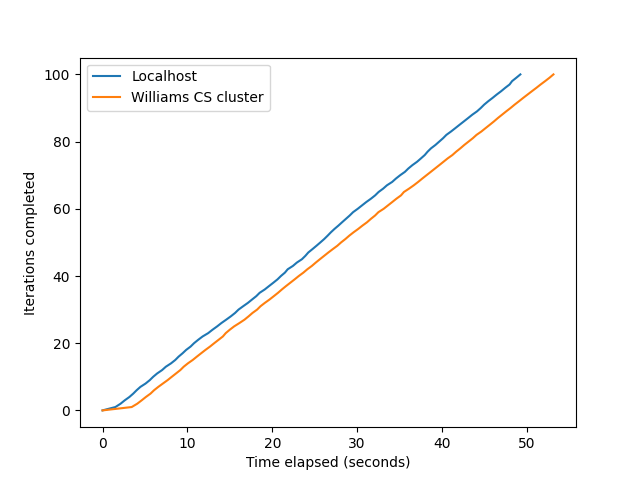
\includegraphics[scale=0.9]{img/experiments/e1_1620966966721.png}
    \caption{Number of iterations completed over time when running \texttt{memory\_usage.shard}.}
    \label{fig:memoryusage}
  \end{center}
\end{figure}

The \texttt{memory\_usage.shard} program was run 100 times sequentially on each of the two clusters.
Figure \ref{fig:memoryusage} shows the number of iterations complete at a given point in time.

In general, the experiment on the localhost cluster acts as a baseline for comparison.
As we can see from the graph, the first iteration of executing the program is slower to complete, as it involves performing some extra computation to set up the connection to the remote machine, and the remainder of the iterations complete at a relatively constant pace for both of the clusters.
When we compare the clusters, the Williams CS cluster takes longer to initiate a connection with, since the endpoints of the connection are on different machines, but overall there is not much of a penalty to using the Williams CS machine cluster, as the network latency is quite small compared to the execution time.
Note that the \texttt{single\_command} application class requires the Shard command to be run on each of the machines in the cluster, so the each iteration on localhost would be expected to complete slightly faster, even with disregarding the network delay of running the programs on a remote machine.


\subsection{Data parallel}
The second experiment in this section verifies that the \texttt{data\_parallel} application class works correctly in producing the expected program output.

\begin{minipage}[c]{\textwidth-15pt}
  \begin{lstlisting}[language=Shard]
# word_count.shard
source cluster_setup.shard
cluster -t data_parallel
cat input.txt |
    tr '[:upper:]' '[:lower:]' |
    tr -cs '[:alnum:]' '\n' |
    (echo $in; echo 1)@@map/testcluster |
    (paste -sd+ - | bc)@@reduce/testcluster
\end{lstlisting}
  \smallskip
\end{minipage}

The program used in this experiment, \texttt{word\_count.shard}, was previously described in the \textbf{Application class: }\texttt{data\_parallel} section of the \textbf{Design} chapter.
This program takes an input from the file \texttt{input.txt} and outputs the number of occurrences for each word present in the file.

The input document for this experiment is Hamlet's Soliloquy (``To be or not to be'') from Shakespeare's Hamlet, which was chosen as an example of a famous passage with a non-trivial amount of repeated words.
This passage has a total of 288 words, which means that each remote machine would have to execute multiple tasks, as opposed to a single task as is the case for the \texttt{memory\_usage.shard} experiment.
The full text of the input document and the expected output can be found in the appendix.

% Experiment (e2)
\begin{figure}[h]
  \begin{center}
    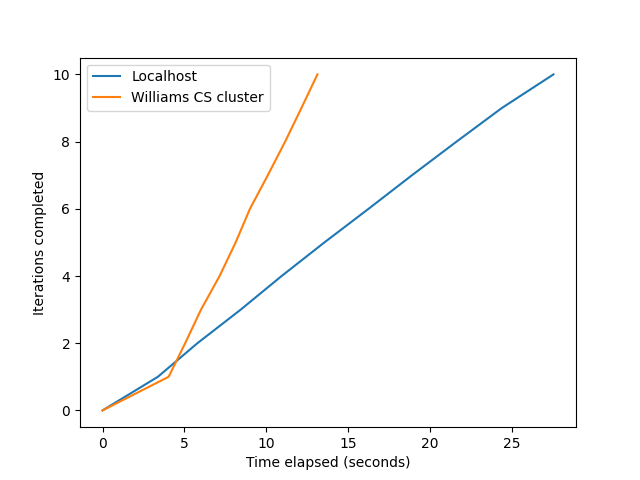
\includegraphics[scale=0.9]{img/experiments/e2_1620960581241.png}
    \caption{Number of iterations completed over time when running \texttt{word\_count.shard}.}
    \label{fig:wordcount}
  \end{center}
\end{figure}

The \texttt{word\_count.shard} program was run 10 times sequentially on each of the two clusters.
Figure \ref{fig:wordcount} shows the cumulative number of trials complete at a given point in time.

As we can see from the graph, the first iteration of executing the program is once again slower to complete due to the setup of Shard.
As opposed when running the \texttt{memory\_usage.shard} script, this time the program completes much faster on the Williams CS cluster when compared to the localhost.
This is because the Williams CS cluster consists of four machines, and the work is divided up among those machines, which lets them process tasks simultaneously, as opposed to having only the local machine itself for the localhost cluster.

\subsection{Data parallel with delay}
The third experiment in this demonstrates Shard's ability to run many tasks in parallel on the same remote machine.
This purpose of this experiment is to demonstrate that Shard's distributed computation capability is extended by its ability to run multiple Shard commands at once, over a single connection, even on the same remote machine, which is achieved by sending the data over a single channel with the Shard network layer, as described in the \textbf{Shard network layer} section of the \textbf{Design} chapter.

\begin{minipage}[c]{\textwidth-15pt}
  \begin{lstlisting}[language=Shard]
# word_count_slow.shard
source cluster_setup.shard
cluster -t data_parallel
cat input.txt |
    tr '[:upper:]' '[:lower:]' |
    tr -cs '[:alnum:]' '\n' |
    (echo $in; sleep 1; echo 1)@@map/testcluster |
    (paste -sd+ - | bc)@@reduce/testcluster
\end{lstlisting}
  \smallskip
\end{minipage}

The program used in this experiment, \texttt{word\_count\_slow.shard} is almost identical to the previous \texttt{word\_count.shard} experiment, except that each \texttt{map} remote command sleeps for 1 second in the middle before its completion.
This program takes an input from the file \texttt{input.txt} and outputs the number of occurrences for each word present in the file.
To simulate a longer-running program with delays in its processing, instead of completing the \texttt{map} portion immediately, a \texttt{sleep 1} command is added to make the program sleep for one second.

This program is expected to take longer to run when compared to \texttt{word\_count.shard}, due to the added sleep command.
However, because multiple remote commands can run simultaneously on the same machine, in a single Shard execution process, a sleeping command does not prevent further commands from being executed, up to a limit based on the number of remote commands that can be ran simultaneously.

% Experiment (e3)
\begin{figure}[h]
  \begin{center}
    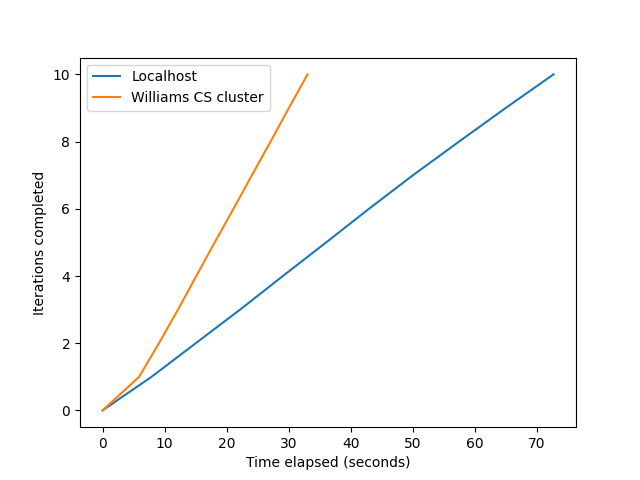
\includegraphics[scale=0.9]{img/experiments/e3_1620960581241.png}
    \caption{Number of iterations completed over time when running \texttt{word\_count\_slow.shard}.}
    \label{fig:wordcountslow}
  \end{center}
\end{figure}

The \texttt{word\_count\_slow.shard} program was run 10 times sequentially on each of the two clusters.
Figure \ref{fig:wordcountslow} shows the cumulative number of trials complete at a given point in time.

This graph looks very similar to the graph for the \texttt{word\_count.shard} program, except that each trial look much longer to complete, due to the delay added to the remote command portion.
However, even though this Shard program runs over 300 total tasks, the amount of time taken to run this program did not increase to over 300 seconds even on the localhost cluster with a single machine.
Once again, note that the \texttt{data\_parallel} application class splits up the task of counting an individual word to the various machines on the cluster, so while the local machine cluster had the lowest latency, it only uses one process to execute remote commands, whereas the remote machine clusters use multiple processes simultaneously (one process to execute the code for each remote machine).
This is especially important because there is a cap to how many simultaneous commands can be ran on a single remote process, which can be quickly reached from many of the remote commands spending a large portion of their time sleeping.

The experiments described in this section collectively show that the Shard distributed framework functions as described in the design section for both the \texttt{single\_command} and \texttt{data\_parallel} application classes.
Producing the correct results for these experiments is a baseline for showing that Shard is a correctly functioning distributed shell programming language.
% Currently, the performance of Shard has not been optimized, so comparable programs written for other distributed systems may be significantly faster than Shard.

Further potential experiments to test the distributed features of the Shard system include testing more complicated programs with multiple remote command invocations on different clusters, including clusters of machines in located in different geographical regions, and running Shard programs on much larger clusters of hundreds or thousands of machines instead of just the handful of machines as used in the experiments here.

\section{Reliable}

% \begin{itemize}
%   \item Still works even in error conditions
%   \item Graph completion time vs random failure rate for \texttt{single\_command} programs with intermittent network errors
%   \item Graph completion time vs random failure rate for \texttt{data\_parallel} programs with both temporarily and permanently failing hosts
% \end{itemize}

After showing that Shard supports distributed computations, the next step is to show that Shard works reliably.
This is what separates Shard from some other systems with naive distributed computing support, as described in the \textbf{Distributed Command-line Shells} section in the \textbf{Background} chapter.

Evaluating Shard for reliability is carried out by running Shard programs over a network, introducing various types of failures that may occur in the real world, and ensuring that Shard manages to complete the computations successfully.
Each experiment also includes a baseline where the failure is not introduced as a point of comparison.
The experiments in this section will measure the the completion progress of several Shard programs over time, showing that the error handling features in Shard are effective at recovering from the failures that are introduced.
For more information on the error handling features of Shard, see the \textbf{Shard network layer} section in the \textbf{Design} chapter.
% The failures being explored in this chapter include trying to connect an unreachable host, remote process crashes, packets being dropped, and slow-running programs.

The cluster of machines used in this section is the same Williams CS cluster as mentioned in the previous section, which consists of four remote machines located on the same local area network as the local machine used to run Shard.
For the experiments in this section, the latest version of Shard is pushed to the remote machines in the cluster before running the experiment, by running a no-op remote Shard program on the cluster, in order to ensure that the results are consistent between the experiments.

The program used in this section for testing the reliability of the \texttt{single\_command} application class is \texttt{random\_hash.shard}, which takes a string of random bytes and computes the MD5 checksum of the input string.

\begin{minipage}[c]{\textwidth-15pt}
  \begin{lstlisting}[language=Shard]
# random_hash.shard
source cluster_setup.shard
(head -c100000000 /dev/urandom | md5sum)@@testcluster
\end{lstlisting}
  \smallskip
\end{minipage}

\begin{sloppypar}
  This program takes one hundred million random bytes from the system random source \texttt{/dev/urandom} and pipes it to the \texttt{md5sum} UNIX program, using the non-cryptographically-secure MD5 hashing algorithm to compute a checksum of the input.
  The purpose of this program is to simulate a computationally expensive program that needs to be reliably executed on each remote machine.
\end{sloppypar}

\begin{sloppypar}
  The program used in this section for testing the reliability of the \texttt{data\_parallel} application class is \texttt{word\_length.shard}, which counts the average length of each word based on the first letter of the word.
\end{sloppypar}

\begin{minipage}[c]{\textwidth-15pt}
  \begin{lstlisting}[language=Shard]
# word_length.shard
source cluster_setup.shard
cluster -t data_parallel
cat input.txt |
    tr '[:upper:]' '[:lower:]' |
    tr -cs '[:alnum:]' '\n' |
    (echo $in | cut -c1;
     echo $in | wc -c)@@map/testcluster |
    (awk '{total += $1}
          END {total/NR}')@@reduce/testcluster |
    sort -t, -nk2 -r
\end{lstlisting}
  \smallskip
\end{minipage}

Parts of this program are identical to the program \texttt{word\_count.shard}, which is previously explained in more depth in the \textbf{Application class: }\texttt{data\_parallel} section of the \textbf{Design} chapter.

\begin{itemize}
  \item
        Line 2, which appears in \texttt{word\_count.shard}, runs the \texttt{cluster\_setup.shard} script to set up the cluster \texttt{testcluster}.
        The cluster of machines used are exclusively the Williams CS machine cluster, composed of remote machines on the same local area network as the local machine. However, the results should still hold for the local machine cluster and the cloud machine cluster.
  \item Lines 3-5, which also appear in \texttt{word\_count.shard}, transform the input into lowercase words separated by newlines.
  \item On lines 6-7 of the program, the input is split up by line and sent to be executed remotely on the cluster \texttt{testcluster}.
        Line 6 outputs the key of the map operation, which uses the \texttt{cut} UNIX program to take the first letter of the word as the key.
        Line 7 outputs the value of the map operation, which uses the \texttt{wc} UNIX program to count the number of letters in the word.
  \item  On lines 8-9 of the program, the input is split up by key, with all values associated with a key sent to be executed remotely on the same machine in the cluster \texttt{testcluster}.
        Lines 8-9 use the \texttt{awk} UNIX program to process the input, which is a list of numbers separated by newlines.
        Line 8 takes each number and adds it to a \texttt{total} variable, and line 9 divides the \texttt{total} value by the \texttt{awk} built-in \texttt{NR}, which is equal to the number of input values seen. This results in outputting the desired value, the average of all inputs.
  \item On line 10 of the program, the remote execution output is passed to the \texttt{sort} UNIX program to sort the output in decreasing average length order.
\end{itemize}
The purpose of this program is to provide another example program that simulates a MapReduce-style data parallel computation similar to the \texttt{word\_count.shard} program, which includes both a custom key and a custom value in the mapping portion, and a post-processing sorting step.

For this section, the \texttt{word\_length.shard} program was run once again on the same input document as previously, which is Hamlet's Soliloquy (``To be or not to be'') from Shakespeare's Hamlet.
The full text of the input document and the expected output can be found in the appendix.

\subsection{Permanently unreachable host}
The first experiment in this section tests the behavior of Shard in the case that a host permanently unreachable.
Examples of real world scenarios that are simulated by this experiment include having a permanent unresolved network failure on a remote host, or typing a host's name in incorrectly during the cluster setup.
The experiment is set up by adding an fifth addition host to the \texttt{cluster\_setup.shard} script that is known to be unreachable, to the four existing machines in the cluster.
The two programs, \texttt{random\_hash.shard} and \texttt{word\_length.shard}, are both run without and with the additional host, and the results of the execution are compared.

\begin{sloppypar}
  When the \texttt{random\_hash.shard} program is run with this additional host, the program consistently hangs forever until interrupted by the user.
  This is due to \texttt{random\_hash.shard} using the \texttt{single\_command} application class, which ensures the remote command completes in a best-effort manner on each remote machine in the cluster.
  As one of the machines in the cluster is unreachable, the application class will continually retry the execution of the remote command, after timing out, because it does not know if the failure to reach the host is due to a temporary or permanent disconnection.
  On the other hand, when running \texttt{random\_hash.shard} without the additional unreachable host, the program reaches completion reliably.
\end{sloppypar}

On the other hand, \texttt{word\_length.shard} is able to successfully complete, even when there is an unreachable host.
This is because \texttt{word\_length.shard} uses the \texttt{data\_parallel} application class, which allows tasks to be allocated to any machine on the cluster, and supports reallocating tasks that fail to complete.

% Experiment (e4)
\begin{figure}[h]
  \begin{center}
    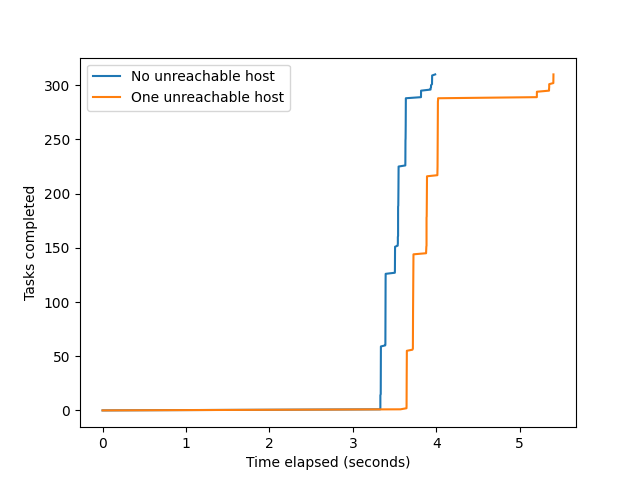
\includegraphics[scale=0.9]{img/experiments/e4_1620960581241.png}
    \caption{Tasks completed over time when running \texttt{word\_length.shard} with and without an unreachable host.}
    \label{fig:unreachable}
  \end{center}
\end{figure}

For \texttt{word\_length.shard}, we look at the number of tasks completed by the cluster over time, where each task completion corresponds to successfully processing either one word in with \texttt{map} operation or one letter with the \texttt{reduce} operation, as is shown in Figure \ref{fig:unreachable}.

The first thing to notice for this graph is that for the first few seconds, no tasks are being completed.
This is because this is the period of time when Shard sets up its connection to the remote machines, and is necessary even when the correct version of Shard is already installed on those machines.

Once this setup is complete, on the cluster with no unreachable hosts, the tasks are completed in the span of less than one second.
However, on the cluster with one unreachable host, the tasks allocated to the one unreachable host cannot be completed, which blocks the progress to completing the Shard program, while the remaining tasks allocated to the four other hosts complete normally.
When Shard detects that one of the hosts is unreachable for a certain timeout, it performs a reallocation of the tasks, using the strategy as described in the \textbf{Remote target selection} section of the \textbf{Design} chapter.
Because the other hosts have a high success rate in completing their tasks, while the unreachable host has a 0\% success rate, all of the tasks are reallocated to the remaining four machines in the cluster, which allows the entire program to promptly complete.
If a random target selection strategy were used instead, it would be very likely that some of the tasks would be reselected for the unreachable host for multiple iterations of timeouts, which would cause the Shard program to take much longer to complete.

If a host is temporarily unreachable, the host will behave in the manner as shown in this experiment for the period in which it cannot be reached. When the host recovers, the remote target selection mechanism will resume sending tasks to this host with low probability until it demonstrates that it is able to consistently complete tasks again.
Although not exactly the same scenario as having a temporarily unreachable host, the next experiment explores when the remote Shard process crashes, and the automatic retry mechanism has to kick in to restart the Shard process on the remote host, so it can continue to process remote tasks.

\subsection{Remote crashes}
The second experiment in this section tests the behavior of Shard in the case that the remote Shard process crashes.
Examples of real world scenarios that are simulated by this experiment include the remote machine running out of memory, or a bug in the Shard runtime results in it crashing.
The two programs, \texttt{random\_hash.shard} and \texttt{word\_length.shard}, are both run without and with crashes, and the results of the execution are compared.

In general, it is very rare for the remote Shard process to crash, because program failures are handled and captured by Shard, and each remote Shard command is executed in an isolated environment.
However, this experiment helps show that even if a remote crash does happen, Shard is still able to recover and continue running the program.

In the case of the \texttt{random\_hash.shard} experiment, the remote machines are set up so that each machine crashes the Shard process a fixed number of times before successfully completing.
This is done by including a \texttt{fixed\_crash.shard} script before running the experiment, using the language feature that allows running local scripts on the remote machine, and passing the number of crashes as the \texttt{crashcount} variable:

\begin{minipage}[c]{\textwidth-15pt}
  \begin{lstlisting}[language=Shard]
# fixed_crash.shard
file=/tmp/shard/crash.txt
if ! [ -a $file ]; then
    echo $crashcount >$file
fi
count=$(cat $file)
if [ $count -ge 1 ]; then
    echo "$count-1" | bc >$file
    killall shard.exe
fi
\end{lstlisting}
  \smallskip
\end{minipage}

\begin{minipage}[c]{\textwidth-15pt}
  \begin{lstlisting}[language=Shard]
# random_hash.shard with forced crashes
source cluster_setup.shard
source -l fixed_crash.shard
for i in 0 1 2 3 4 5; do
    crashcount=$i
    (rm -f /tmp/shard/crash.txt)@@testcluster
    (source -r fixed_crash.shard;
    head -c100000000 /dev/urandom | md5sum)@@testcluster
done
\end{lstlisting}
  \smallskip
\end{minipage}

The \texttt{fixed\_crash.shard} program checks if a file named \texttt{/tmp/shard/crash.txt} exists on the remote machine.
If \texttt{crash.txt} file does not exist, it is initialized with the crash count as specified by the \texttt{crashcount} variable.
Then, the program reads and updates the file's contents as a numerical input, indicating the number of crashes left on this machine.
As long as there is at least one crash remaining, the program uses the \texttt{killall} UNIX command to crash the Shard process.

% Experiment (e5)
\begin{figure}[h]
  \begin{center}
    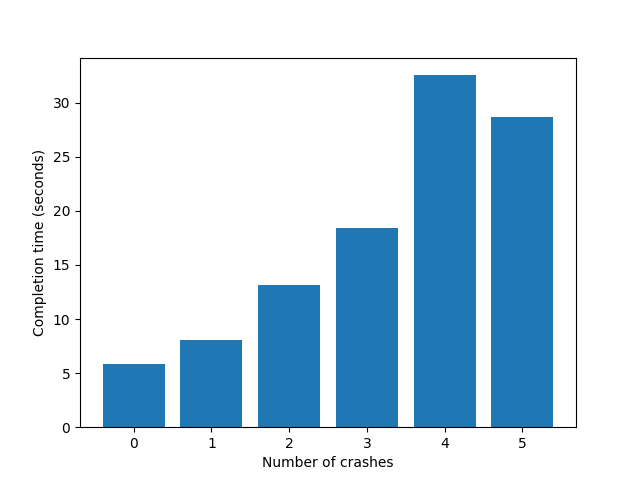
\includegraphics[scale=0.9]{img/experiments/e5_1620960581241.png}
    \caption{Time taken to run \texttt{random\_hash.shard} based on the number of forced crashes on each remote machine}
    \label{fig:crashhash}
  \end{center}
\end{figure}

The \texttt{random\_hash.shard} experiment was run six times, with the number of crashes on each remote machine varying from 0 to 5.
Figure \ref{fig:crashhash} shows the time it takes for the program to complete, based on the crash count of each remote machine.

From this graph, we can see that as the number of forced crashes increases, so does the time it takes to complete the program by a large amount.
This is because, whenever Shard crashes on the remote machine, the local instance of Shard must detect the crash and reinitialize a new instance of Shard on the remote machine, which is an expensive operation.
However, because this graph only shows the result of running this experiment a single time, some random noise caused the completion time of running the program with 4 crashes to end up being longer than running the program with 5 crashes.

The remote crashes experiment is also run on the \texttt{word\_length.shard} program.
This time, rather than having all remote Shard processes deterministically crashing a fixed number of times, instead, there is random chance for each remote job to crash the remote process.
This is done by including a \texttt{random\_crash.shard} script before running the experiment:

\begin{minipage}[c]{\textwidth-15pt}
  \begin{lstlisting}[language=Shard]
# random_crash.shard
rand=$(shuf -i 1-100 -n 1)
if [ $rand -le $crashpercent ]; then
    killall shard.exe
fi
\end{lstlisting}
  \smallskip
\end{minipage}

The \texttt{random\_crash.shard} program uses the \texttt{shuf} UNIX command to randomly generate a number between 1 and 100, inclusive.
This value is compared to the crash percent, as passed in to this program with the variable \texttt{\$crashpercent}.
If the randomly generated value is less than or equal to the crash percent, the \texttt{killall} UNIX command is used to crash the Shard process.

% Experiment (e6)
\begin{figure}[h]
  \begin{center}
    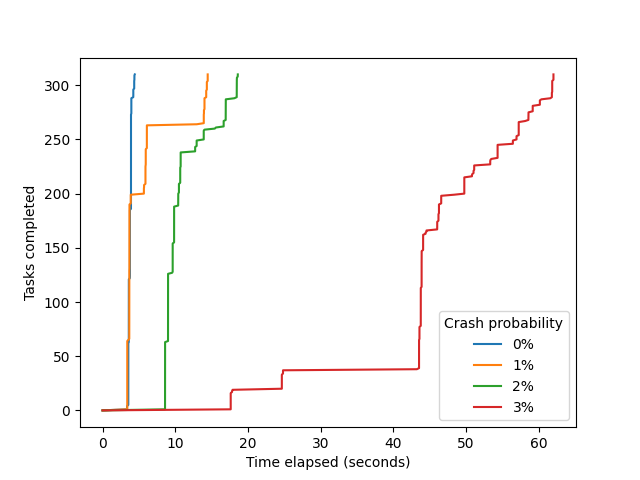
\includegraphics[scale=0.9]{img/experiments/e6_1620960581241.png}
    \caption{Tasks completed over time when running \texttt{word\_length.shard} based on the chance for a job to randomly crash.}
    \label{fig:crashwordlength}
  \end{center}
\end{figure}

The \texttt{word\_length.shard} experiment was run four times, with the probability of a crash ranging from 0 to 3 percent for each task executed, but uniform for all machines in any particular trial.
Figure \ref{fig:crashwordlength} shows the time it takes for the program to complete, based on the crash chance of each remote machine.

From this graph, we can see that even a slight increase in the crash probability can have a massive impact in slowing down the program's completion.
This is largely because when a remote machine crashes in a \texttt{data\_parallel} program, not only does the task associated with the crash fail to complete, but so do all of the other tasks running on the same machine.
These failed tasks might only be discovered as failed when they do not complete within a certain timeout period.
Because many tasks run in parallel on each of the remote machines in the cluster, the chance that one or more of them end up crashing the Shard process on that machine is likely, even when the chance of any given task causes a crash is small.
Nevertheless, Shard is able to recover from the remote Shard process unexpectedly crashing many times, which shows the resilience of the Shard distributed framework to severe disruptions.

\subsection{Program failure}
The third experiment in this section tests the behavior of Shard in the case of a remote program failing, by explicitly exiting with a non-zero exit code.
An example of a real world scenario that is simulated by this experiment is when the remote Shard program encounters some unrecoverable situation and the best strategy is to retry the entire remote task rather than recover in some other fashion.
The program failure is simulated by modifying the script to randomly call the \texttt{exit} builtin with a nonzero exit code in a similar fashion to the random Shard crashing simulated with the previous experiment.
The program \texttt{word\_length.shard} is run with different chances of random program failure, and the results are compared.

A program failing is very similar to the case of a Shard process crashing, with the key difference being that Shard crashing is more disruptive -- rather than losing all progress on currently executing tasks on the remote machine and having to restart the remote process, the Shard network layer can communicate that the remote task has failed, and a retry can be issued by the Shard network layer immediately on the same remote process.
This means that the time to completion for failing programs should be lower than for crashing processes.

\begin{sloppypar}
  The random failure experiment is run on the \texttt{word\_length.shard} program, in an experiment very similar to the random crash experiment for \texttt{word\_length.shard}.
\end{sloppypar}

% Experiment (e8)
\begin{figure}[h]
  \begin{center}
    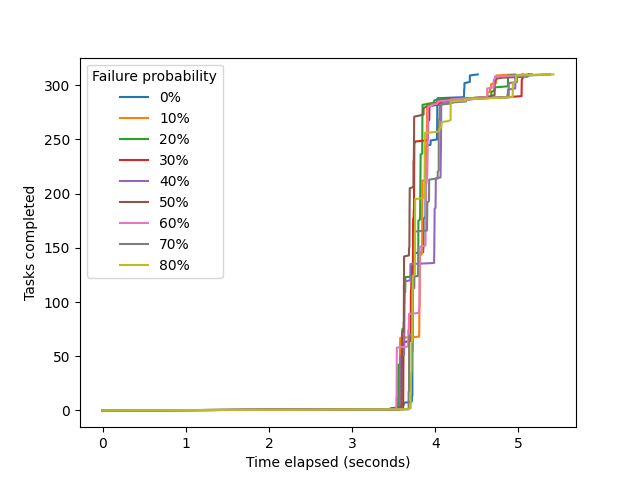
\includegraphics[scale=0.9]{img/experiments/e8_1620960581241.png}
    \caption{Tasks completed over time when running \texttt{word\_length.shard} based on the chance for a job to randomly fail.}
    \label{fig:failwordlength}
  \end{center}
\end{figure}

The \texttt{word\_length.shard} experiment was run nine times, with the chance of random failure varying from 0 percent to 80 percent for each trial, but uniform for all machines in any particular trial.
Figure \ref{fig:failwordlength} shows the average time it takes for the program to complete execution on a specific remote machine, based on the failure rate of that machine.

From this graph, we can see that Shard manages to complete quickly, even when the probability that a given task fails is very high -- the time taken to complete the program with 80\% failure is less than 2 seconds longer than the time taken to complete the program with 0\% failure.
This is in stark contrast with the results of the previous experiment that explores the circumstance when the remote Shard instance crashes.
The reason why a Shard task failing is not very disruptive is that the local Shard instance can immediately know when the task fails, because this information is communicated through the Shard network layer.
As such, failing tasks can be immediately detected and rescheduled to a machine in the cluster with no penalty except for the time it took to run that task.
Even so, when this program is run with a high enough failure probability that approaches 100\%, the program can still end up taking very long to complete.

\subsection{Data loss}
The fourth experiment in this section tests the behavior of Shard in the case that packets used by the Shard network layer are randomly lost.
An example of a real world scenario that is simulated by this experiment is when part of the data being transferred is lost due to network errors.
The two programs, \texttt{random\_hash.shard} and \texttt{word\_length.shard}, are run with different chances of random Shard network layer packet loss, and the results are compared.
The data loss is simulated by modifying Shard's local receiver code to randomly drop incoming network layer packets, depending on the currently set packet loss rate.

For the execution of a Shard program, the impact of data loss is closer to the impact of Shard crashing than to the impact of a program failure, as it is difficult to detect when to reschedule a task due to data loss, because it may be possible that the task will send that data at some point in the future, which can significantly delay the rescheduling of tasks.
Similar to random crashes, it is generally unlikely for this packet loss issue to occur in practice, but this experiment helps show that even when Shard network layer packet loss does occur, Shard is able to correctly handle the error.

For the \texttt{random\_hash.shard} program, most of the packets sent back to the local machine are heartbeat packets, indicating that the program is still alive.
Depending on the timeout parameters, if some number of heartbeat packets are dropped, the retry mechanism is triggered, which may affect the rate of completion of the overall program.
Note that even in the circumstance of a retry, if the original program comes back with a good response, it will be accepted.
The most important packets not to be lost in this execution are the data packet, which contains the hash result, and the close packet, indicating that the remote execution is complete.
If the close packet is lost, the remote program is never marked as complete.
If the data packet is lost, the sequence number mechanism prevents the close packet from being accepted.

% Experiment (e9)
\begin{figure}[h]
  \begin{center}
    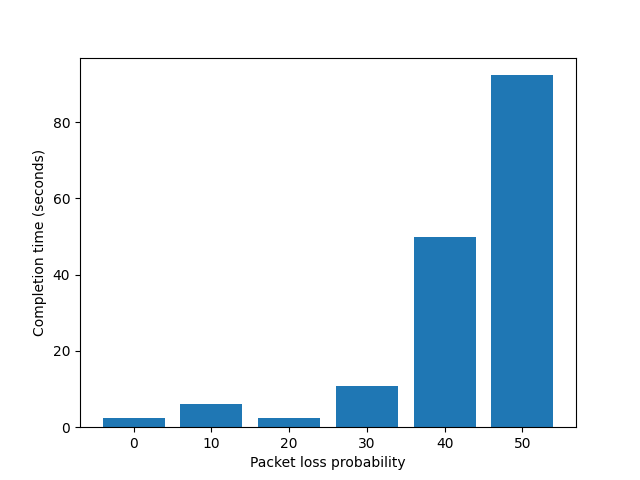
\includegraphics[scale=0.9]{img/experiments/e9_1620960581241.png}
    \caption{Time taken to run \texttt{random\_hash.shard} for different packet loss rates.}
    \label{fig:packetlosshash}
  \end{center}
\end{figure}

The \texttt{random\_hash.shard} program was run six times for the packet loss probabilities ranging from 0\% to 50\%, with the same packet loss rate being applied to all of the machines in the cluster on any given trial.
Figure \ref{fig:packetlosshash} shows the completion time of each trial for the various packet loss rates.
Note that the packet loss is randomly applied, which explains why the completion time did not always increase when the packet loss rate did.

As we can see from this graph, a higher probability of packet loss can cause the program to take significantly longer to complete.
This is because a typical Shard program sends back many packets to the local instance of Shard, and each of the data packets and close packets must be received by the local instance of Shard for the task to be marked as completed.
If any of these packets are dropped, the remote execution must be retried, which can result in many retries for the same task.
Shard ensures that it receives all packets that it sends by using the sequence number mechanism as described in the \textbf{Task cluster abstraction} section in the \textbf{Design} chapter.

The experiment involving the \texttt{word\_length.shard} program will be slightly different from each of the previous experiments, in that it tests the scenario where the machines in the cluster have different probabilities of encountering an error.

% For the \texttt{word\_length.shard} program, many more packets are sent overall.
% If some packets are lost, the retry mechanism will reexecute the task, potentially on a different machine.

% Experiment (e10)
\begin{figure}[h]
  \begin{center}
    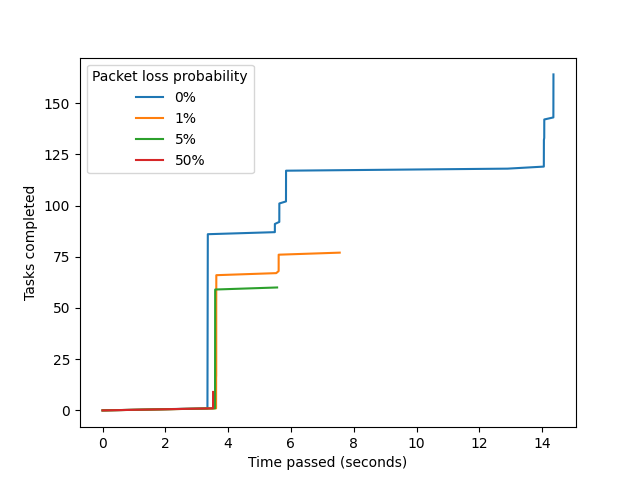
\includegraphics[scale=0.9]{img/experiments/e10_1620960581241.png}
    \caption{Tasks completed over time when running \texttt{word\_length.shard} by each machine in a cluster with the machines having different packet loss probabilities.}
    \label{fig:packetlosswordlength}
  \end{center}
\end{figure}

The \texttt{word\_length.shard} program was run on the Williams CS cluster with four machines, where the probability that a packet is loss on the four machines were 0\%, 1\%, 5\%, and 50\%.
Figure \ref{fig:packetlosswordlength} shows the of number of tasks completed over time by each of the machines in the cluster.
Note that for this figure and for the next figure, each line represents the number of tasks completed by a single machine, as opposed to all machines in a trial.

In the first few seconds, the connection is established to each remote machine, and tasks are distributed to all of the machines in the cluster.
However, each of the machines completes a different number of tasks before grinding to a halt, due to the dropped packets resulting in incomplete tasks.
After a period of timeout of around 2 seconds, the incomplete tasks are rescheduled, with the proportion of tasks being allocated to each machine in the cluster based on its previous success rate.
The bump at the 6 second mark shows that even taking the lower probability of success into account, most tasks were being allocated to the cluster with no data loss, and almost no tasks were being allocated to the cluster with 50\% packet loss.
This helps Shard complete its execution significantly faster when compared to randomly allocating tasks each time.
More information can be found in the \textbf{Remote target selection} section of the \textbf{Design} chapter.
Eventually, the machine with 0\% packet loss is used to complete all of the remaining tasks, because it has demonstrated that it is significantly more likely for a task to be completed when using that machine.

\subsection{Slow computation}
The fifth experiment in this section tests the behavior of Shard in the case that certain machines are consistently slower to complete their tasks.
Examples of real world scenarios simulated by this experiment are when certain machines on a cluster are overloaded or unresponsive due to running too many tasks, or when a partial hardware failure causes a machine to be running at a handicapped rate.

% Experiment (e11)
\begin{figure}[h]
  \begin{center}
    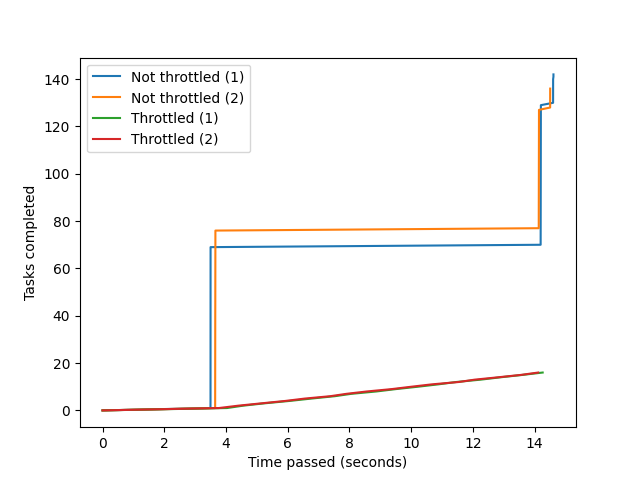
\includegraphics[scale=0.9]{img/experiments/e11_1620960581241.png}
    \caption{Tasks completed over time when running \texttt{word\_length.shard} by each machine in a cluster with some machines rate-limited.}
    \label{fig:slowwordlength}
  \end{center}
\end{figure}

For this experiment, the \texttt{word\_length.shard} program was run on the Williams CS cluster with four machines.
The first two machines are ``fast'' machines, which behave normally and have no restrictions on rate of processing tasks.
The latter two machines are ``slow'' machines, which have a restriction that only one task can be processed at a time on the machine, and tasks take an additional 0.5 seconds longer to process.
Figure \ref{fig:slowwordlength} shows the cumulative number of jobs completed by each of the machines in the cluster after a certain point in time.
% Because the first two machines in the cluster are much faster at completing tasks, more tasks end up being scheduled to these machines, which improves the overall performance of the entire program.

As this graph shows, the tasks allocated to the two ``fast'' machines that are not throttled are completed within a second, while the tasks allocated to the two ``slow'' throttled machines take much longer to complete.
After a certain timeout, even though the two throttled machines are successfully completing tasks, the remaining tasks allocated to those machines are reallocated, using the remote target selection mechanism.
This mechanism uses the information that the two ``fast'' machines are able to successfully complete all of the tasks allocated to them, and that the two ``slow'' machines have yet to complete many of its tasks, to decide to schedule a vast majority of the remaining tasks to the ``fast'' machines.
This means that, even though the two ``slow'' machines are not strictly speaking failing to complete tasks, the reallocation allows the entire program to be completed in a much shorter timespan by deprioritizing the ``slow'' machines when allocating tasks.

\section{Easy to use}

% \begin{itemize}
%   \item Provide examples of sample programs
%   \item If time permits, ask other programmers (potentially with less knowledge on distributed systems/programming languages) to try writing programs
%   \item Line of code/code size comparisons?
%   \item only 2 new forms of syntax
%   \item write equivalent to SSH program
% \end{itemize}

Finally, Shard is evaluated for its core pillar of being easy to use.
Unlike the evaluation for the other core pillars, this section does not involve using experiments and measuring performance.
Rather, it provides a set of explanations that justify the ease of use of Shard, using comparisons to existing solutions for additional justification.

\subsection{Setup}

Being easy to use begins with the procedure to set up the system in the first place.
The following steps were used to set Shard up for the Williams CS machine cluster:
\begin{enumerate}
  \item Setup SSH access to each remote machine from the local machine (this step was already completed before starting the Shard project, because SSH access is useful outside of the scope of Shard).
        \begin{enumerate}
          \item Generate an SSH key pair on the local machine for the entry point.
          \item Add the SSH private key to the SSH agent on the local machine.
          \item Add the SSH public key to the known hosts on each remote machine.
        \end{enumerate}
  \item Obtain the Shard executable.
  \item Write a script setting up the cluster of machines, using the \texttt{cluster} builtin. This involves giving the cluster a name, and adding the hosts to the cluster.

        \begin{minipage}[c]{\textwidth-25pt}
          \begin{lstlisting}[language=Shard]
# cluster_setup.shard for Williams CS cluster
# Hostnames here differ from the ones used in the actual experiment
cluster -s testcluster
cluster -a machine1.cs.williams.edu
cluster -a machine2.cs.williams.edu
cluster -a machine3.cs.williams.edu
cluster -a machine4.cs.williams.edu
\end{lstlisting}
          \smallskip
        \end{minipage}

  \item Run the Shard executable.
  \item Include the cluster setup script with the \texttt{source} builtin.

        \begin{minipage}[c]{\textwidth-25pt}
          \begin{lstlisting}[language=Shard]
source cluster_setup.shard
\end{lstlisting}
          \smallskip
        \end{minipage}

  \item Write a one line program to run a remote command on the cluster.

        \begin{minipage}[c]{\textwidth-25pt}
          \begin{lstlisting}[language=Shard]
(uname -a)@@testcluster
\end{lstlisting}
          \smallskip
        \end{minipage}

\end{enumerate}

Other than setting up SSH access, all steps of the setup were performed on the local machine where Shard is running, and each step only supplies the necessary information needed by Shard to run the remote command.
In addition, for running future Shard programs on the same machine, steps 1-3 only need to be completed again if the set of machines in the cluster changes.
When setting up Shard, there is no need to
\begin{itemize}
  \item copy files manually to remote machines;
  \item run scripts manually on remote machines;
  \item run additional daemon scripts;
  \item obtain root access on any machine;
  \item change security settings;
  \item check for existing installations of Shard;
  \item set up a configuration file, other than the cluster setup, which provides the necessary information of which remote hosts to add to the cluster;
  \item perform any other additional setup.
\end{itemize}

\subsection{Writing Shard programs}

The Shard programming language is easy to learn for someone with only passing familiarity of another POSIX shell programming language because it has a very minor set of additions compared to the POSIX shell specification.

Programmers only need to know about two features of Shard to utilize its remote execution capabilities, as these are the only additions to the Shard programming language:
\begin{itemize}
  \item the remote execution infix operator, \texttt{@@}
  \item the \texttt{cluster} builtin.
\end{itemize}
If the user wants to take advantage of the additional functionality provided by Shard's application classes, the user only needs to learn about how they work on a surface level.

As an example, assume that the user wants to write a Shard script that uses the \texttt{data\_parallel} application class, and that the user has already set up a \texttt{cluster\_setup.shard} script to define a cluster \texttt{testcluster}.
The user wants to write a script that finds the length of each line of an input file, \texttt{input.txt}, and calculates the number of occurrences for each of the line lengths present.

The first step is to import the \texttt{cluster\_setup.shard} script, and set the application class of the cluster to \texttt{data\_parallel}, which is achieved by two Shard builtins.

\begin{minipage}[c]{\textwidth-15pt}
  \begin{lstlisting}[language=Shard]
source cluster_setup.shard
cluster -t data_parallel
\end{lstlisting}
  \smallskip
\end{minipage}

The next step is to figure out what the specifics of the map and reduce operations in order to solve the problem.
For this problem, because the goal is to find the number of occurrences grouped by line length, the key of the map operation should be the line length.
Since the value should be a simple count, each instance in the input contributes 1 to the count, so the value of the map operation should be 1.
Note the syntax for the remote execution:
\begin{itemize}
  \item The program to be executed remotely is surrounded by parentheses, where the syntax within is identical to a shell program, making the process analogous to invoking a subshell;
  \item The \texttt{@@} operator is located directly after the closing parentheses;
  \item After the \texttt{@@} operator, the ``target'' is specified. In this case, the target is running the remote program with the \texttt{map} operation on the cluster \texttt{testcluster}. Here, \texttt{map} is a special string used by the \texttt{data\_parallel} application class, and may vary depending on which application class the cluster utilizes.
\end{itemize}

\begin{minipage}[c]{\textwidth-15pt}
  \begin{lstlisting}[language=Shard]
source cluster_setup.shard
cluster -t data_parallel
(wc -c $in; echo 1)@@map/testcluster
\end{lstlisting}
  \smallskip
\end{minipage}

The reduce operation aggregates the values for each key, which is a list of 1's equal to the number of occurrences.
Therefore, to get the total number of occurrences for each key, a shell command to find the sum of the input should be used for the reduce operation.
Because of how the \texttt{data\_parallel} application class is designed, the output of the map operation is piped to the input of the reduce operation.

\begin{minipage}[c]{\textwidth-15pt}
  \begin{lstlisting}[language=Shard]
source cluster_setup.shard
cluster -t data_parallel
(wc -c $in; echo 1)@@map/testcluster |
    (paste -sd+ - | bc)@@reduce/testcluster
\end{lstlisting}
  \smallskip
\end{minipage}

Finally, the input text comes from the text file \texttt{input.txt}, which should be piped as input to the map operation to complete the program, \texttt{line\_length.shard}.

\begin{minipage}[c]{\textwidth-15pt}
  \begin{lstlisting}[language=Shard]
# line_length.shard
source cluster_setup.shard
cluster -t data_parallel
cat input.txt |
    (wc -c $in; echo 1)@@map/testcluster |
    (paste -sd+ - | bc)@@reduce/testcluster
\end{lstlisting}
  \smallskip
\end{minipage}

Here, we have shown that, by reasoning about the functionality of the program, it is reasonably straightforward to write the Shard program, with only a basic understanding of the additions of Shard needed.

We can compare the above to the following shell program, \texttt{line\_length\_ssh.sh}, that utilizes SSH to perform the same task in counting the occurrences of each line length in a distributed fashion.
The specifics of the program will not be explained in detail.
Notably, however, this implementation in shell is much more complicated (we can simply compare the line and character counts between the two programs), while lacking the features and the reliability provided by the Shard runtime.

\lstset{xleftmargin=15pt}
\begin{lstlisting}[language=bash]
# line_length_ssh.sh
# Define hosts of machine in cluster
m1=machine1.cs.williams.edu
m2=machine2.cs.williams.edu
m3=machine3.cs.williams.edu
m4=machine4.cs.williams.edu

# Cleanup from prior runs
rm -f map_*.txt
rm -f all_keys.txt
rm -f unique_keys.txt
rm -f result.txt

# Map function
map () {
    # Choose a random host
    # Note that the POSIX shell does not support arrays
    target=$(echo -e "$m1\n$m2\n$m3\n$m4" | shuf -n 1)
    # Execute map job on remote host
    result=$(echo "" | ssh "$target" "(echo \"$1\" | wc -c; echo 1)")
    # Retreive the key
    key=$(echo "$result" | head -n 1)
    # Retreive the value
    value=$(echo "$result" | tail -n 1)
    # Generate the output file depending on the key
    outfile="map_$key.txt"
    # Replace newline with comma, and append to temporary file
    echo "$value" >> $outfile
    # Keep track of the set of all keys
    echo "$key" >> all_keys.txt
}

# Reduce function
reduce () {
    # Choose a random host
    # Note that the POSIX shell does not support arrays
    target=$(echo -e "$m1\n$m2\n$m3\n$m4" | shuf -n 1)
    # Generate the input file depending on the key
    infile="map_$1.txt"
    # Execute reduce job on remote host
    result=$(cat "$infile" | ssh "$target" "(paste -sd+ - | bc)")
    # Print result to the standard output
    echo "$line,$result" >> result.txt
}

# Map operation
# Loop through each line of the input
# Make sure to read last line if the file does not end in EOF
while IFS= read -r line || [[ -n "$line" ]]; do
    # Asynchronously call the map function, which executes a map task
    map "$line" &
done < input.txt

# Wait for tasks to complete
wait

# Deduplicate key list
sort all_keys.txt | uniq > unique_keys.txt

# Reduce operation
# Loop through each key
# Make sure to read last line if the file does not end in EOF
while IFS= read -r line || [[ -n "$line" ]]; do
    # Asynchronously call the reduce function, which executes a reduce task
    reduce "$line" &
done < unique_keys.txt

# Wait for tasks to complete
wait

# Sort results
sort -t, -nk1 result.txt
\end{lstlisting}
\lstset{xleftmargin=0pt}

% Experiment (e12)
\begin{figure}[h]
  \begin{center}
    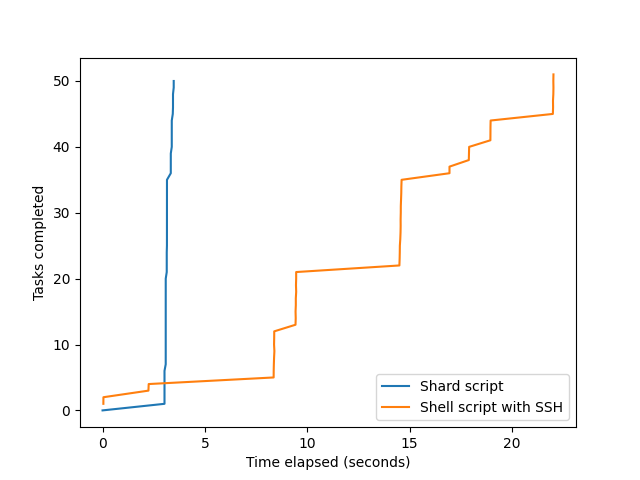
\includegraphics[scale=0.9]{img/experiments/e12_1621061398991.png}
    \caption{Tasks completed over time when running \texttt{line\_length.shard} on Shard versus \texttt{line\_length\_ssh.sh} on Bash.}
    \label{fig:linelength}
  \end{center}
\end{figure}

\begin{sloppypar}
  The two programs, \texttt{line\_length.shard} and \texttt{line\_length\_ssh.sh}, are each run with the input of Hamlet's Soliloquy (``To be or not to be'') from Shakespeare's Hamlet, with \texttt{line\_length.shard} running in Shard, and \texttt{line\_length\_ssh.sh} running in the Bash shell.
  The full text of the input document and the expected output can be found in the appendix.
  Figure \ref{fig:linelength} shows the number of tasks completed by \texttt{line\_length.shard} and \texttt{line\_length\_ssh.sh} over time.
  Note that the \texttt{line\_length\_ssh.sh} script is slightly modified so it reports the elapsed time whenever a task is completed.
\end{sloppypar}

As we can see from this graph, the Shard script completes much faster than the equivalent Bash script.
Both the Shard script and the Bash script attempt to schedule jobs in parallel.
However, the primary difference between the two programs that causes the Shard script to complete significantly faster is that the Bash script requires setting up a new SSH connection to the remote machine for each remote task execution.
In addition, when running the experiment, the Bash script failed several times before completing successfully, due to errors caused by making too many SSH connections at once.
The errors can be avoided by modifying the Bash scripts to run the tasks synchronously rather than in parallel, at the cost of taking much longer to complete the tasks.
It is possible to work around these limitations, but the resulting code would be even more complicated than it already is, especially compared to the simplicity of the equivalent Shard script.

In addition to being easy to create a new Shard program from scratch, it is also easy to port an existing shell program to Shard, adding remote execution functionality in the process.
At the most basic level, a valid shell program is also a valid Shard program, with some caveats that the current implementation of Shard does not have all of the features as defined by the POSIX shell specification, nor many of the additional features in various shell implementations.
Even if the original program does not support remote execution, such support can be added incrementally, with each intermediate program being a valid Shard program.

\subsection{Error recovery}

Shard's ease of use is also demonstrated in the circumstance that an error occurs in the execution of the remote program.
As shown in the \textbf{Reliable} section of this chapter, Shard is capable of automatically handling many different types of failures that may arise when using a distributed system, including unreachable remote hosts, process crashes, program failures, data loss, and slow-running remote machines.
These would not be handled if the user were using SSH on an existing shell, unless the user adds special case-specific code to handle each of the situations previously described.
This means that, in the case that one of the failure circumstances does arise, using Shard's automatic error detection and recovery mechanisms is much easier than trying to figure out where and why the failure occurred.
As an example, let's say the user is trying to run a cleanup task on each of the machines in some cluster \texttt{remotes} with hundreds of machines, and print out a success message, as defined in the \texttt{cluster.shard} script.

\begin{minipage}[c]{\textwidth-15pt}
  \begin{lstlisting}[language=Shard]
source cluster.shard
(rm -r /tmp/cache_to_be_removed; echo "$(hostname) - cleanup success")@@remotes
\end{lstlisting}
  \smallskip
\end{minipage}

Without using Shard, if a remote single machine on the cluster is unreachable, the program may immediately fail and not try to continue on the remaining machines, or even worse, the failure may be silently ignored.
When Shard is used, the reliable execution behavior of the \texttt{single\_command} application class results in retrying the task if a failure occurred, until it succeeds or the user exits Shard.
If Shard is exited without completing the task on all hosts, the success message will print exactly once on the remote hosts where the command executed, allowing the user to accurately figure out on which machines the command did not execute, in spite of multiple retries.
This example shows a practical real-world scenario where the error recovery built into Shard is useful in helping Shard achieve its ease of use.

\section{Summary}

In this section, we describe a set of experiments used to evaluate the design and implementation of Shard, in how well it satisfies the core pillars of Shard.

Example \texttt{single\_command} and \texttt{data\_parallel} programs run with various remote machine clusters to demonstrate that Shard works seamlessly over a network, satisfying the core pillar of being distributed.

More example programs are run, with distributed systems errors deliberately being introduced, to show that Shard automatically handles various failures that may arise when running remote programs, satisfying the core pillar of being reliable.

Finally, a qualitative analysis of setting up Shard, writing Shard programs, and recovering from errors automatically in Shard provide evidence that Shard satisfies the core pillar of being easy to use.

\chapter{Conclusion}
% \begin{itemize}
%   \item Research question
%   \item Solution (design, implementation)
%   \item Measuring success (three pillars)
%   \item Future work
%   \item What did this thesis accomplish?
% \end{itemize}

In this thesis, we explore the research question of how to create a reliable and easy to use general purpose distributed framework.
This thesis proposes the Shard distributed framework, which provides a solution that satisfies the three goals of being distributed, reliable, and easy to use, which we deem as the three core pillars of Shard.
Many existing computer systems achieve some of these goals, but to our knowledge, none of them satisfy all of the core pillars to the extent that Shard does.

Shard builds on the POSIX shell programming language by adding a small set of language and syntax additions to create a new programming language that supports executing remote subprograms within a Shard program.
Using the concept of application classes, which describe a set of semantics for remote execution, it is possible to write many different types of distributed programs with different properties in Shard.
A network layer designed specifically for Shard provides the functionality of running remote Shard programs, and ensures that remote tasks are executed in a reliable way.

This thesis describes a specific implementation of Shard using the OCaml programming language, the way that the various parts of Shard are structured in the implementation, and how the implementation can be easily extended to add additional language features or application classes.

Shard is evaluated by running experiments to demonstrate that the design and implementation satisfy the core pillars. The experiments show that, with the programs being tested, Shard does an excellent job in functioning as a general purpose reliable distributed shell programming language, while still maintaining the ease of use in setting up Shard, writing Shard code, and running Shard programs.

There are many possible directions to extend this work.
Some of them include peer-to-peer communication between remote machines in a cluster, compatibility on different architectures, performance improvements, alternative language features, and additional application classes.
Many of these directions can be investigated by extending the existing implementation of Shard as provided by this thesis, but it is also viable to create an alternative implementation with different trade-offs.

% \todoi{Future: Lesson learned}

Shard offers a glimpse to the future of distributed programming, where, with a few minutes of setup, any programmer can write an ad hoc script that executes reliably on a cluster of remote machines, without needing to learn all of the intricacies of programming for a distributed system.


\chapter{Appendix}
\section{Appendix A: Example program input and output}

\subsection{A1. Input text: Hamlet's Soliloquy from Shakespeare's Hamlet}

Source: Project Gutenburg \cite{hamlet}.

\lstset{xleftmargin=15pt}
\begin{lstlisting}[language=]
To be, or not to be, that is the question:
Whether 'tis nobler in the mind to suffer
The slings and arrows of outrageous fortune,
Or to take arms against a sea of troubles,
And by opposing end them? To die—to sleep,
No more; and by a sleep to say we end
The heart-ache, and the thousand natural shocks
That flesh is heir to: 'tis a consummation
Devoutly to be wish'd. To die, to sleep.
To sleep, perchance to dream—ay, there's the rub,
For in that sleep of death what dreams may come,
When we have shuffled off this mortal coil,
Must give us pause. There's the respect
That makes calamity of so long life.
For who would bear the whips and scorns of time,
The oppressor's wrong, the proud man's contumely,
The pangs of dispriz'd love, the law's delay,
The insolence of office, and the spurns
That patient merit of the unworthy takes,
When he himself might his quietus make
With a bare bodkin? Who would these fardels bear,
To grunt and sweat under a weary life,
But that the dread of something after death,
The undiscover'd country, from whose bourn
No traveller returns, puzzles the will,
And makes us rather bear those ills we have
Than fly to others that we know not of?
Thus conscience does make cowards of us all,
And thus the native hue of resolution
Is sicklied o'er with the pale cast of thought,
And enterprises of great pith and moment,
With this regard their currents turn awry
And lose the name of action. Soft you now,
The fair Ophelia! Nymph, in thy orisons
Be all my sins remember'd.
\end{lstlisting}

\subsection{A2. Output from \texttt{word\_count.shard}}

\begin{lstlisting}[language=]
a,5
ache,1
action,1
after,1
against,1
all,2
and,12
arms,1
arrows,1
awry,1
ay,1
bare,1
be,4
bear,3
bodkin,1
bourn,1
but,1
by,2
calamity,1
cast,1
coil,1
come,1
conscience,1
consummation,1
contumely,1
country,1
cowards,1
currents,1
d,4
death,2
delay,1
devoutly,1
die,2
dispriz,1
does,1
dread,1
dream,1
dreams,1
end,2
enterprises,1
er,1
fair,1
fardels,1
flesh,1
fly,1
for,2
fortune,1
from,1
give,1
great,1
grunt,1
have,2
he,1
heart,1
heir,1
himself,1
his,1
hue,1
ills,1
in,3
insolence,1
is,3
know,1
law,1
life,2
long,1
lose,1
love,1
make,2
makes,2
man,1
may,1
merit,1
might,1
mind,1
moment,1
more,1
mortal,1
must,1
my,1
name,1
native,1
natural,1
no,2
nobler,1
not,2
now,1
nymph,1
o,1
of,15
off,1
office,1
ophelia,1
opposing,1
oppressor,1
or,2
orisons,1
others,1
outrageous,1
pale,1
pangs,1
patient,1
pause,1
perchance,1
pith,1
proud,1
puzzles,1
question,1
quietus,1
rather,1
regard,1
remember,1
resolution,1
respect,1
returns,1
rub,1
s,5
say,1
scorns,1
sea,1
shocks,1
shuffled,1
sicklied,1
sins,1
sleep,5
slings,1
so,1
soft,1
something,1
spurns,1
suffer,1
sweat,1
take,1
takes,1
than,1
that,7
the,22
their,1
them,1
there,2
these,1
this,2
those,1
thought,1
thousand,1
thus,2
thy,1
time,1
tis,2
to,15
traveller,1
troubles,1
turn,1
under,1
undiscover,1
unworthy,1
us,3
we,4
weary,1
what,1
when,2
whether,1
whips,1
who,2
whose,1
will,1
wish,1
with,3
would,2
wrong,1
you,1
\end{lstlisting}

\subsection{A3. Output from \texttt{word\_length.shard}}

\begin{lstlisting}[language=]
q,8.5
c,8.3
r,7.71429
p,6.75
u,5.83333
e,5.75
g,5.66667
f,5.5
s,5.41667
m,5.28571
n,5.1
k,5
h,5
d,5
w,4.95238
l,4.83333
t,4.5
o,4.5
b,4.23077
a,4.14815
i,4.125
y,4
\end{lstlisting}

\subsection{A4. Output from \texttt{line\_length.shard}}

Note that the shell script \texttt{line\_length\_ssh.sh} produces the same output.

\begin{lstlisting}[language=]
27,1
37,1
38,2
39,2
40,5
41,1
42,4
43,5
44,2
45,4
46,1
48,2
49,2
50,2
52,1
\end{lstlisting}

%%%%%%%% References %%%%%%%%%%
\bibliographystyle{acm}
\bibliography{references}
%%%%%%%% End References %%%%%%

\end{document}
